
\documentclass[a4paper]{article}

% CJK support: prefer ctex, fallback to XeTeX native line breaking
\IfFileExists{ctex.sty}{
  \usepackage[fontset=fandol]{ctex}
}{
  \usepackage{fontspec}
  \XeTeXlinebreaklocale "zh"
  \XeTeXlinebreakskip = 0pt plus 1pt
  \IfFontExistsTF{Songti SC}{\setmainfont{Songti SC}}{%
    \IfFontExistsTF{Noto Serif CJK SC}{\setmainfont{Noto Serif CJK SC}}{}%
  }
  \IfFontExistsTF{Heiti SC}{\setsansfont{Heiti SC}}{%
    \IfFontExistsTF{Noto Sans CJK SC}{\setsansfont{Noto Sans CJK SC}}{}%
  }
}

\usepackage{amsmath, amssymb}
\usepackage{graphicx}
\usepackage[margin=2.5cm]{geometry}
\usepackage[most]{tcolorbox}
\usepackage{etoolbox}
\usepackage{listings}
\usepackage{hyperref}
\usepackage{booktabs}
\usepackage{subcaption}
\usepackage{float}
\usepackage{tikz}

\newtcolorbox{knowledgebox}[1]{
    enhanced, colback=blue!5!white, colframe=blue!75!black, colbacktitle=blue!75!black,
    coltitle=white, fonttitle=\bfseries, title=#1, attach boxed title to top left={yshift=-2mm, xshift=2mm},
    boxrule=1pt, sharp corners
}

\newtcolorbox{importantbox}[1]{
    enhanced, colback=yellow!10!white, colframe=yellow!80!black, colbacktitle=yellow!80!black,
    coltitle=black, fonttitle=\bfseries, title=#1, sharp corners
}

\newtcolorbox{warningbox}[1]{
    enhanced, colback=red!5!white, colframe=red!75!black, colbacktitle=red!75!black,
    coltitle=white, fonttitle=\bfseries, title=#1, sharp corners
}

\lstset{
    basicstyle=\ttfamily\small,
    keywordstyle=\color{blue},
    stringstyle=\color{red!60!black},
    commentstyle=\color{green!60!black},
    breaklines=true,
    frame=single,
    numbers=left,
    numberstyle=\tiny\color{gray},
    captionpos=b,
    extendedchars=false
}

\newcommand{\vtag}{\protect\footnotemark}
\newcommand{\srcnote}[1]{\footnotetext{视频画面时间区间：#1。若为裁剪图，时间区间仍对应原视频画面。}}
\newcommand{\degC}{\ensuremath{^{\circ}\mathrm{C}}}
\newcommand{\um}{\ensuremath{\mu\mathrm{m}}}
\newcommand{\nm}{\ensuremath{\mathrm{nm}}}
\newcommand{\angstrom}{\ensuremath{\text{\AA}}}

\newcommand{\notetitle}{软件仓库管理}
\newcommand{\notesubtitle}{从目录、快照到 AI 时代的工程约定 —— 南京大学《生成式软件工程》第 3 讲}
\newcommand{\noteauthors}{lecture-to-notes 整理}
\newcommand{\notedate}{\today}
\newcommand{\videochannel}{绿导师原谅你了（南京大学 · 生成式软件工程）}
\newcommand{\videopublishdate}{2026-09-08}
\newcommand{\videoduration}{1 小时 40 分 13 秒}
\newcommand{\videourl}{https://www.bilibili.com/video/BV1kybV6DE47/}
\newcommand{\videocoverpath}{cover.jpg}

\begin{document}

\begin{titlepage}
\centering
{\Large 课程笔记\par}
\vspace{1.2cm}
{\huge\bfseries \notetitle\par}
\vspace{0.3cm}
{\large \notesubtitle\par}
\vspace{0.5cm}
{\large \noteauthors\par}
\vspace{0.3cm}
{\large \notedate\par}
\vspace{1.0cm}

\includegraphics[width=0.82\textwidth,height=0.40\textheight,keepaspectratio]{\videocoverpath}\par

\vfill
\begin{tcolorbox}[width=0.9\textwidth, colback=black!2!white, colframe=black!60, sharp corners]
\textbf{视频作者/频道}：\videochannel\par
\textbf{发布日期}：\videopublishdate\par
\textbf{视频时长}：\videoduration\par
\textbf{视频链接}：\href{\videourl}{\nolinkurl{\videourl}}
\end{tcolorbox}
\end{titlepage}

\tableofcontents
\newpage

%% --- 正文内容开始 --- %%

\section{开场：AI 时代还要不要学软件工程}

\subsection*{本节回答的问题}
在模型能力快速上涨的当下，一条“把不顺心挡掉”的 AI 工作流，是否已经替代了学习软件工程基础的需要？

\subsection{一段梗图引出的差距}

课程用一张梗图开场：GPT-6 发布后，“当你被导师 pressure 说上周什么都没做，你突然想起了一个不属于你的力量”。讲者顺势复盘了这个假想模型的观感：编程能力提升有限，倒是生成更快、更适合做复杂任务；而“有经验的软件工程师有品位，这个品位能否指导 AI 做出更好的东西”仍然没被解决——“现在 AI 更多的时候是完成任务”，讲者自嘲“我经常还要骂它，所以我觉得我可能还能再苟活几个月”。

这个调侃指向本课反复使用的一组概念：intent（意图）、specification（规范）与 implementation（实现）之间的空间。同样一句“给我做一个国民级应用”，不同产品经理脑中的目标并不相同，AI 无法与人脑直接对齐，只能按自己的方式漂移。为什么模型“做得不好”的时刻，恰好都出现在这个开放空间里，是整门课的技术底色之一。

\begin{figure}[H]
\centering
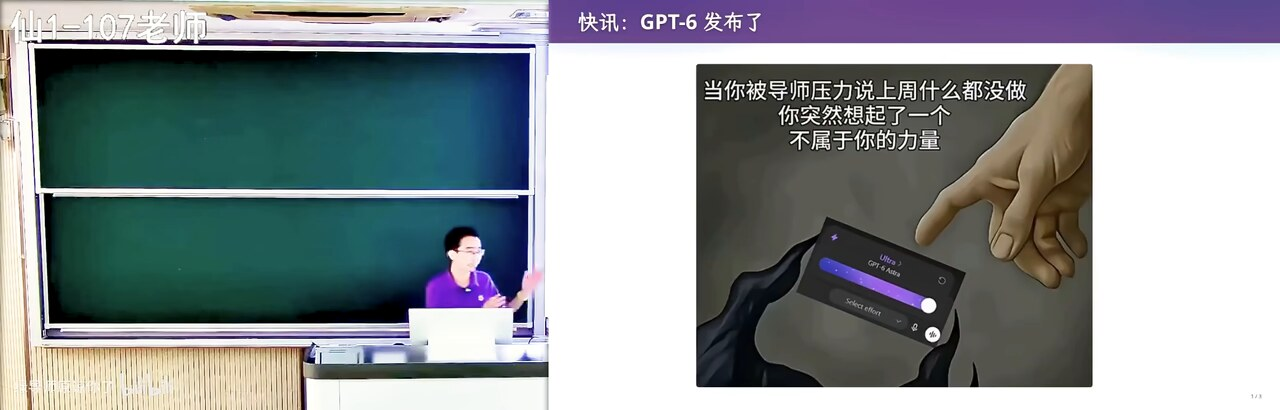
\includegraphics[width=\textwidth]{figures/fig_01_gpt6_meme.jpg}
\caption{开场梗图：GPT-6 发布与“不属于你的力量”，AI 被寄望替你挡住一切不顺心\vtag}
\end{figure}
\srcnote{00:00:00--00:00:14}

幻灯片随即把问题学术化：一个“好用的界面”，什么叫好用往往看到第一版才说得清；实现还会反过来改变需求——设计过程中题目本身在变。讲者引用 Herbert Simon 在 1973 年的论断：结构良好与结构不良的问题之间，边界是流动的，开放的问题也能逐步变得可求解\footnote{Simon, H. A. (1973). The structure of ill structured problems.}。把 spec--impl 空间“越推越窄”，正是软件工程方法与 AI 协同工作的共同目标。

\begin{figure}[H]
\centering
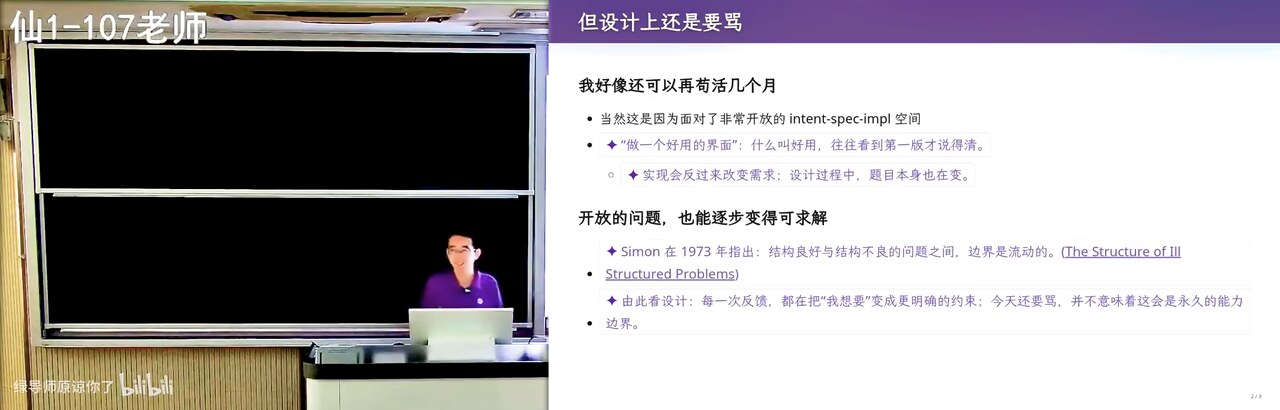
\includegraphics[width=\textwidth]{figures/fig_02_spec_impl_simon.jpg}
\caption{spec--impl 开放空间：Simon（1973）指出结构良好与结构不良问题的边界是流动的\vtag}
\end{figure}
\srcnote{00:01:00--00:01:14}

\subsection{为什么讲者相信模型会继续变强}

讲者转述了他对 OpenAI 路线的理解：先让 AI 学会数学，因为数学是“人类世界里最难的语言”，却拥有全球一致的推理系统——一个定理对不对，全世界都能验证。这与软件工程中 intent/spec/implementation 的 GAP 恰好相反：数学天然可 grounding，而需求没有共识。数学能力再向其他能力辐射：空间想象（鲁班锁、骰子展开图这类可以从简单任务开始做强化学习的题）已经被证明能练出来，随后是具身控制——语言模型不解锁特殊提示词，逐帧问“下一步干什么”，机械臂抓取和叠衣服就达到 state of the art。讲者的博士生做了小半年 3D 生成工作，被新版模型 one-shot 直出“杀死比赛”，是他判断“模型一定会进步”的个人证据。这段判断属于讲者对产业趋势的预期，不是实验结论，本课保留其不确定性。

\subsection{汽车类比：还要不要学}

被反复问到的问题：“AI 时代还要不要学数据库、操作系统？”讲者的回答分两层。早期汽车开一两千公里就出故障，司机必须懂发动机；今天的自动驾驶让“开到某地”变成一句话，人已经完全不理解系统怎样工作，却照样到达目的地。AI 类似汽车但更强——它替代的不只是腿，还有智力。讲者的结论是明确的“要学”，理由却与传统的“打基础”不同：学了以后“你可以更好地解锁 AI 的创造力”，理解了正确的概念，才能从别处借鉴知识来创造新东西；至于“以后应该怎么学”，他说自己暂时没有答案，欢迎讨论。这是讲者的个人立场，他也坦承这种立场并不特别确定。

\begin{figure}[H]
\centering

\includegraphics[width=\textwidth]{figures/fig_03_learn_why.jpg}
\caption{"Anyway…我们还是要学习的”：专家知识围绕核心概念组织（引 How People Learn, 2000），今天进入真正的软件工程任务\vtag}
\end{figure}
\srcnote{00:07:15--00:07:29}

幻灯片给出的学习论依据来自《How People Learn》（2000）：专家的知识围绕核心概念组织，这种组织方式支持在新情境中运用知识。它预告了本课的组织方式——不背命令，而是从需求把概念一个个推出来。

\subsection{本章小结}

模型会变强、执行会被外包，这两点讲者都当作前提接受；他留给读者的问题是：当执行力便宜了，\emph{正确的概念}还值不值钱。他的答案是值钱，而且更值钱——因为它决定你能不能指挥 AI。下一节先把“软件工程的项目”这个最小单元讲清楚：它只是一个目录。

\section{项目就是一个目录：从 U 盘到 Git}

\subsection*{本节回答的问题}
一个软件工程项目到底是什么？在 Git 之前，人们怎样管理它的变化，为什么那些方式注定失败？

\subsection{目录、文件与可交付的东西}

不做作业、不下载模板，真正开始一个项目的第一步是建一个目录，起个名字（比如“我最酷的 JavaGame 软件工程”）。目录里混着 intent、spec、impl 与测试用例，经过 build 或运行得到可交付的东西：一个 \texttt{npm run dev} 起的本地窗口，或者一个双击即开的 exe。

\begin{figure}[H]
\centering
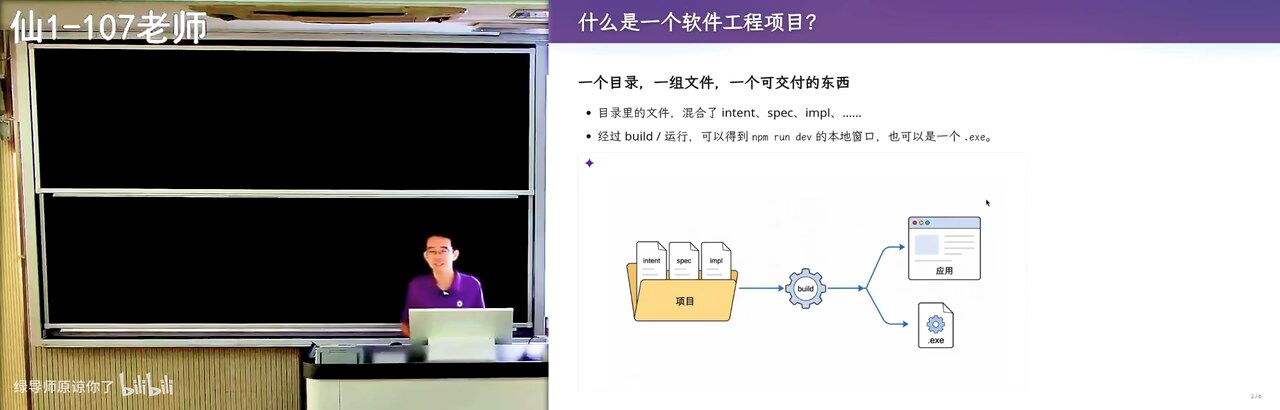
\includegraphics[width=\textwidth]{figures/fig_04_project_directory.jpg}
\caption{软件工程项目 = 一个目录 + 一组文件 + 一个可交付的东西；intent/spec/impl 混在同一目录里\vtag}
\end{figure}
\srcnote{00:09:45--00:09:59}

“软件是什么”这个老先生们爱问的问题，在这里有了实用版答案：代码、文档等一切相关物的集合；讲者自己的表述更形象——软件是人类世界的需求在信息世界的一个投影，投影今天的样子就是一个目录。软件无处不在的佐证来自教室：连脚下这张升降桌都靠软件才能升降，屏幕一角显示当前高度是 106 厘米。

一个 localhost 的笑话说明了“知识”与“意图”的耦合：让 agent 帮你运行程序，弹出的窗口只存在于 \texttt{localhost}，全世界其他人都打不开——除非你在文档里把“要被全世界看到”写进 intent，否则模型会把你当开发者，先起本地开发服务器。知识会累积成目录结构里的默认做法，这也是后面 Git 一切约定的人文本源。

\subsection{古早时期：一个 U 盘装全部代码}

讲者回忆第一个博士生（约 2012 年入学）的故事：大一嫌笔记本屏幕小，去机房写代码，用 U 盘来回拷贝；大二 U 盘坏了，代码全没了。讲者自己上学时交作业的方式是打一个压缩包发邮件。他强调“甚至 10 年以前大家真的是这样的”——保存靠介质，历史靠人脑。

\begin{figure}[H]
\centering
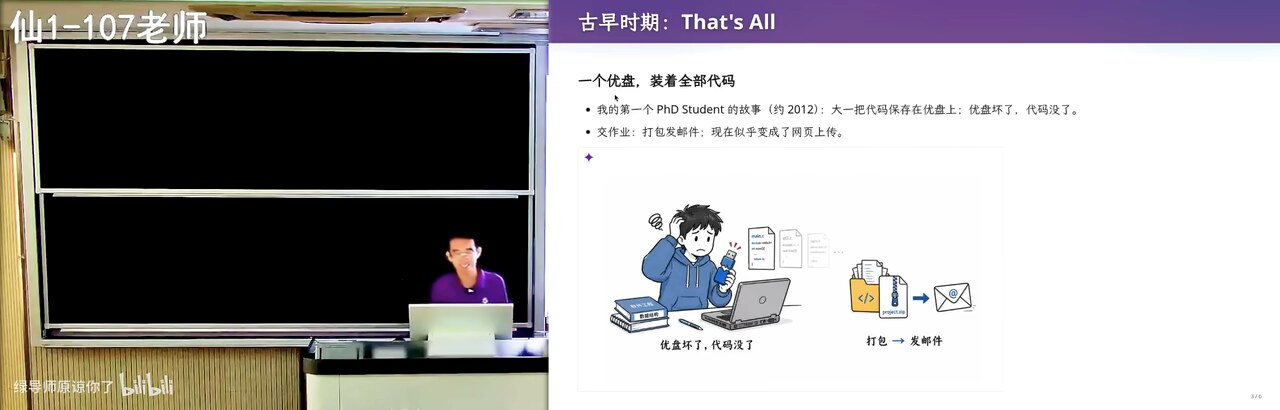
\includegraphics[width=\textwidth]{figures/fig_05_usb_era.jpg}
\caption{古早时期：U 盘装着全部代码，坏了就归零；交作业打包发邮件\vtag}
\end{figure}
\srcnote{00:14:45--00:14:59}

\subsection{今天：版本管理有了标准答案}

今天谈软件工程，保存项目有标准答案：用 Git。它除了保存目录当前状态，还能\emph{保留、比较和恢复}历史版本。课程工作流也因此标准化：\texttt{git clone} 获取作业项目，\texttt{git pull} 获取后续更新，\texttt{make submit} 打包提交到课程网站——由项目里的 Makefile 定义的提交入口，接近一个小型 CI/CD（讲者预告 CI/CD 会专门讲一次）。

\begin{figure}[H]
\centering
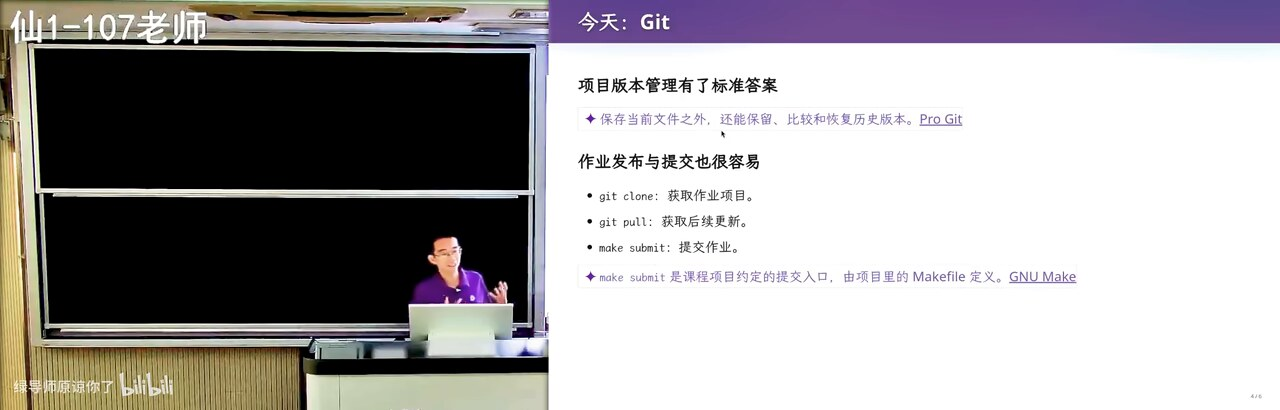
\includegraphics[width=\textwidth]{figures/fig_06_today_git.jpg}
\caption{今天：Git 是项目版本管理的标准答案；clone/pull/make submit 构成课程作业闭环\vtag}
\end{figure}
\srcnote{00:15:15--00:15:29}

\begin{importantbox}{项目与仓库}
项目是一个目录：代码、文档、intent、spec、测试用例混在一起，经构建产生可交付物。版本管理回答的问题只有一个：\textbf{目录在任意过去时刻的样子，能不能被保留、比较、恢复}。Git 之前的所有方案，都是对这一句话的不同折衷。
\end{importantbox}

\subsection{本章小结}
项目 = 目录。目录会改、会改错，于是需要“回到过去”的能力。U 盘和邮件把这份能力外包给介质和人品；Git 把它变成工具的内建性质。下一节暂时离开工具，谈一个更前置的问题：同样刷过几十个 GitHub 项目，为什么有人学到了东西，有人没有。

\section{学习意识：注意力是软件工程的入口}

\subsection*{本节回答的问题}
信息密度远超课堂的时代，怎么把“看过”变成“学会”？

\subsection{别人的项目就是你的学习素材}

讲者几乎每节课都重复这件事：你们都看过很多 Git 项目——哪怕只是打开课程作业，它也带着 GitHub 链接。有的项目有这个文件，有的没有；有的文档这样写，有的那样写。这些信号不断进入时，人本应自动形成判断。现实是中学心态的延续：“老师说要做的我才会做”，像被强化学习成“老师说做这件事就绝不多碰一点”的新手 AI——讲者提醒，AI 被调成这样，人也把自己调成了这样。

反例练习：看到满世界由超长 README、Unicode 字符画的目录框图组成的“AI slop”之后，突然点进一个维护了十几年的老项目——README 很短，想看的三个链接就在眼前。两种体验一对比，“文档应该怎么写”就自动学会了。讲者接着给出城市路牌的观察：在香港，每当前方有三个岔口，正前方一定有路牌告诉你三个口分别是什么；而在南京的地铁站，你常常要走很远找到一张全局地图。好的界面设计遵循同一个原则：\emph{用最少的方式，把决策需要的全部信息放在决策点}。

\begin{figure}[H]
\centering

\includegraphics[width=\textwidth]{figures/fig_07_learning_awareness.jpg}
\caption{学习意识：大量别人的项目就是学习素材；“上课耽误学习”的本质是信息密度与使用方法的落差\vtag}
\end{figure}
\srcnote{00:21:15--00:21:29}

\subsection{“先自己解一遍”的读法}

读论文的老话“virtually implement”被推广到一切课程：面对一个具体问题，先在脑中自己做一遍，再看作者做法。一致，说明你已经掌握；不一致，若是作者更精巧，就问为什么，让它变成你的知识；若你的更好（大约一万次一次），那就是惊喜中的惊喜，正反馈极大。读 Git 项目、读 AI 生成的代码，同样先问“如果是我，我会怎么组织”，再比较谁更好——觉得“我做得更好”的时刻，就是识别 slop 的时刻。

\begin{figure}[H]
\centering
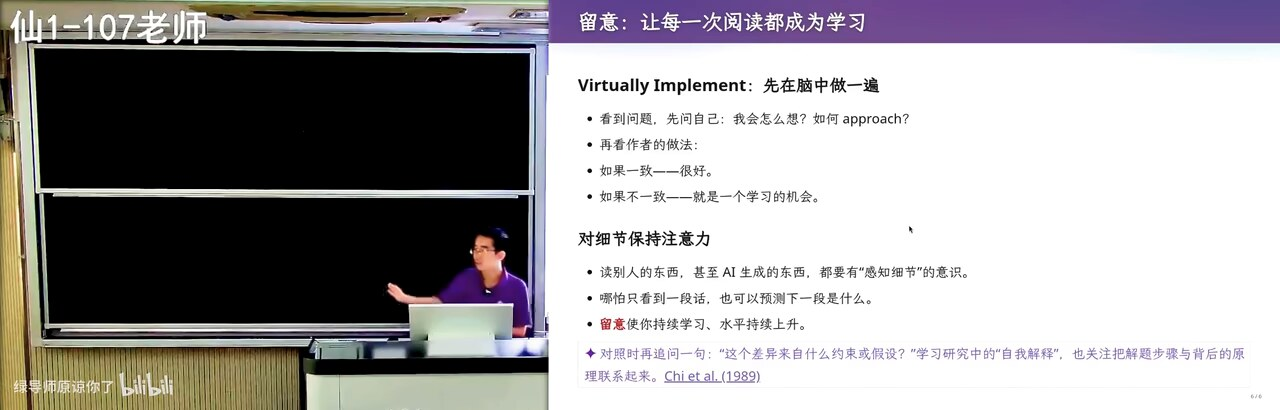
\includegraphics[width=\textwidth]{figures/fig_08_attention_detail.jpg}
\caption{对细节保持注意力：先自己解一遍，再对照作者的做法，把不一致变成学习机会\vtag}
\end{figure}
\srcnote{00:22:15--00:22:29}

\begin{knowledgebox}{路牌原则}
每当用户面临选择，就在选择点给全所需信息。香港地铁的岔口路牌是空间版；Git 把冲突双方的内容直接写进文件是代码版；好的 README 只放三个你要的链接是文档版。原则统一，场景不同。
\end{knowledgebox}

\subsection{本章小结}
工具再强，学习发生在“先自己想一想，再对比”的间隙里。为了检验这种意识是否真的存在，讲者拿自己上周的保研面试做了一次现场实验——下一节就是实验结果。

\section{一次面试当试纸：冲突暴露了“用过”与“听说过的”差距}

\subsection*{本节回答的问题}
把 Git 用进工作流的人，与只“听说过”Git 的人，差别会在哪个具体场景暴露？

\subsection{面试实录}

推免面试上，讲者问了三个问题。第一问“什么是 Git”，多多少少都能答：从 GitHub 下载分发代码，有人能说到目录快照，这在意料之内、可以给过。第二问“git rebase 是什么”，答卷是刺眼的 0/10，而且在意料之外。第三问“git merge 发生冲突以后，你会观察到什么”，竟无人答出那个关键事实：文本冲突时，双方内容和冲突标记会被\emph{直接写进工作区文件}，\texttt{git status} 显示 both modified。

\begin{figure}[H]
\centering
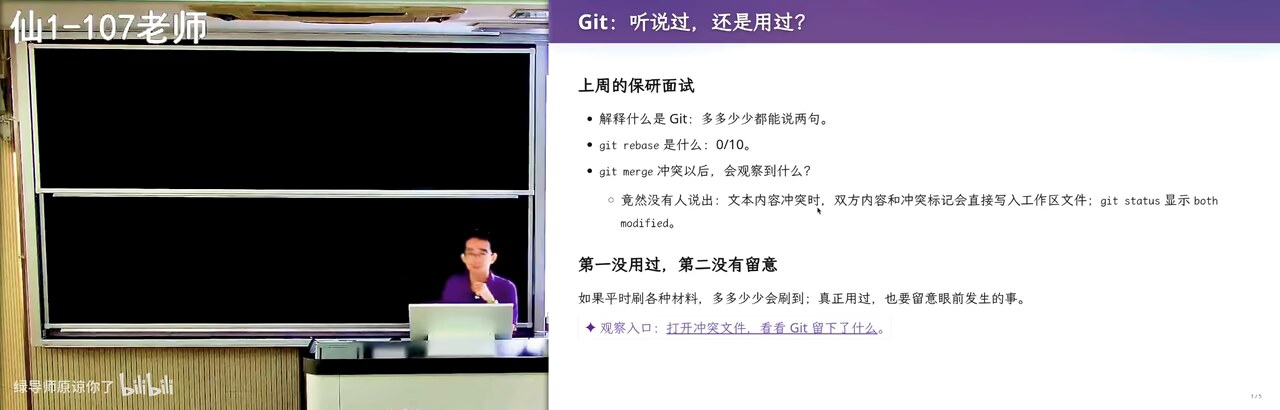
\includegraphics[width=\textwidth]{figures/fig_09_interview_git.jpg}
\caption{保研面试实录：Git 概念人人能说两句，rebase 与冲突观察大面积答不出\vtag}
\end{figure}
\srcnote{00:25:15--00:25:29}

讲者的诊断只有两行：第一，没用过——即使全程让 agent 开发，在不同分支让 agent 干活也很容易遇到冲突；第二，没留意——让 agent 一句“来，帮你修好了”，冲突处理过程整个被代理掉了，眼前发生的事从未进入视野。

\subsection{冲突是责任机制，不是故障}

站在 Git 设计者的角度：文件 1111，一人把第二行改成 2，另一人改成 3，工具无法替你决定以谁为准。Git 选择不躺平，也绝不擅自合并，而是把冲突现场原样呈现——把责任交回每个开发者手里；发现冲突并解决它，是版本控制契约的一部分。于是有了冲突标记这种“把信息堆在决策点”的设计：\texttt{<<<<<<<}、\texttt{=======}、\texttt{>>>>>>>} 把双方内容同时写进文件；IDE 再补上 Accept Incoming / Current Change 按钮；处理完重新提交，冲突即被 resolve。

\begin{warningbox}{{“Agent 说修好了”的盲区}}
让 agent 处理冲突时，它可能悄悄选择了某一侧、或机械合并双方改动。冲突标记写进文件本来是给人看的，人若从没看过，就既不知道自己放弃了什么，也无法在事后审计。至少亲手处理过一次冲突，才算第一次真正“用过”Git。
\end{warningbox}

\subsection{本章小结}
面试数据说明：多数人把 Git 当下载器，没有把它当“历史的审计工具”。要理解这些机制为什么长这样，最有效的方式是从需求重新发明它们——下一节先回到 Git 之前的世界，看看人类在版本管理上真正走错的是哪一步。


\section{Git 之前的世界：三种模型与 Linux 的故事}

\subsection*{本节回答的问题}
版本管理工具是怎么被需求一步步逼出来的？上一个“标准答案”SVN 输在哪里？

\subsection{先把旧的留下来}

最直觉的方案是复制整个目录：作业-v1、作业-v2、作业-最终版。它能找回旧文件，但“哪份从哪份改来、谁改了什么”全靠人记。再往前一步是 RCS 这类工具：替你保存文件的历史版本。多人协作登场后，CVS、SVN 把历史集中放在一台服务器，大家 check out 取文件、修改、check in 交回。Git 的差别在于：保存项目的一个个版本，同时记录版本之间的来路，帮助多人汇合改动——通常每个人本地就持有完整历史。

\begin{figure}[H]
\centering
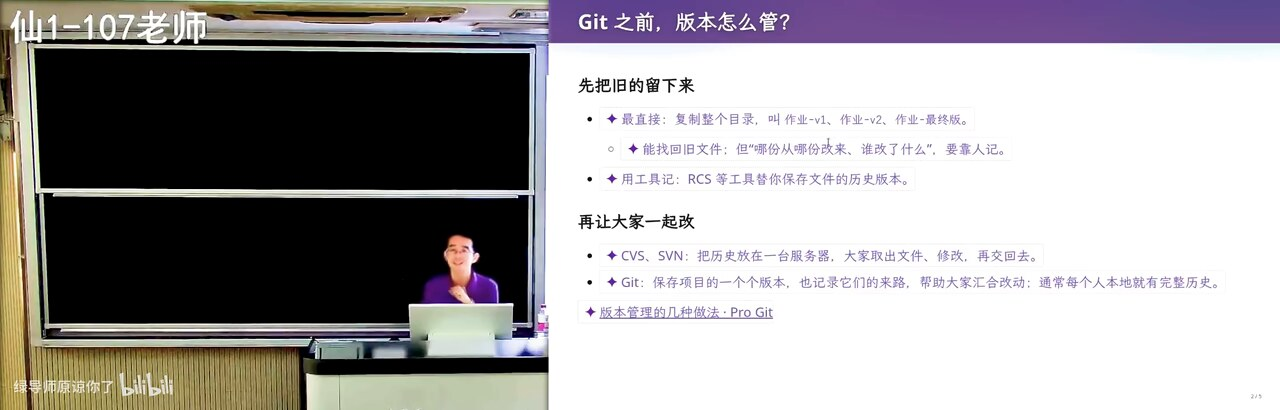
\includegraphics[width=\textwidth]{figures/fig_10_pre_git_era.jpg}
\caption{Git 之前：目录复制、RCS、CVS/SVN 到 Git 的两步演化——先留住旧版本，再让大家的改动汇合\vtag}
\end{figure}
\srcnote{00:30:00--00:30:14}

\begin{center}
\small
\begin{tabular}{llll}
\toprule
方案 & 历史放在哪 & 存储内容 & 回到旧版本的代价 \\
\midrule
目录复制（作业-v1/v2） & 人的记忆 & 每版全量目录 & 找到对应目录即可 \\
RCS & 服务器/本机 & 文件历史版本 & 逐文件恢复 \\
CVS / SVN & 中心服务器 & \textbf{增量 patch} & 沿链逐个倒带 \\
Git & 每人本地（完整） & \textbf{版本快照+来路} & 一步检出 \\
\bottomrule
\end{tabular}
\end{center}

\subsection{走错的一步：存增量}

SVN 与 Git 的根本分歧在存储模型。SVN 说：我存项目的\emph{变化}——最初版本加一串 patch，改一行存一个 patch。这是非常高效的实现，但随着项目增长，高效反而把大家拖进泥潭：想回到一个早期版本，就得沿增量链一个一个往回退（当然可以用缓存类方法优化）。Git 的 first principle 则干净得多：

\begin{equation}
\text{rewind}(v_k)\;=\;
\begin{cases}
\Theta(k), & \text{增量模型：沿 } k \text{ 个 patch 逐个反向应用}\\[2pt]
\Theta(1), & \text{快照模型：直接检出 } v_k \text{ 的根对象}
\end{cases}
\end{equation}
式中 \(k\) 为目标版本距最新版本的提交数；\(\Theta(k)\) 表示代价随链长线性增长；快照模型下任何版本都同样近。

讲者认为“确实走错路了”，Git 的作者（Linux 的作者）要的是“绝对简单、概念正确，又非常好用”的工具。

\subsection{Linux 内核：一个大项目逼出自己的工具}

1991 到 2002 年，维护 Linux 的方式就是“作业-v1/v2 + 邮件列表”：开发者改一个 \texttt{a.c}，把新版直接发到邮件列表；maintainer 看到补丁，放进自己的核心仓库，再 release。2002 年，内核团队采用商业工具 BitKeeper 管理多人并行开发，免费使用权后来被收回。2005 年，Linus 等人开发了自己的工具——Git 由此诞生，比大多数人想象的年轻。需求其实一直都在：保存来路，让许多人的改动汇成一个项目。

\begin{figure}[H]
\centering
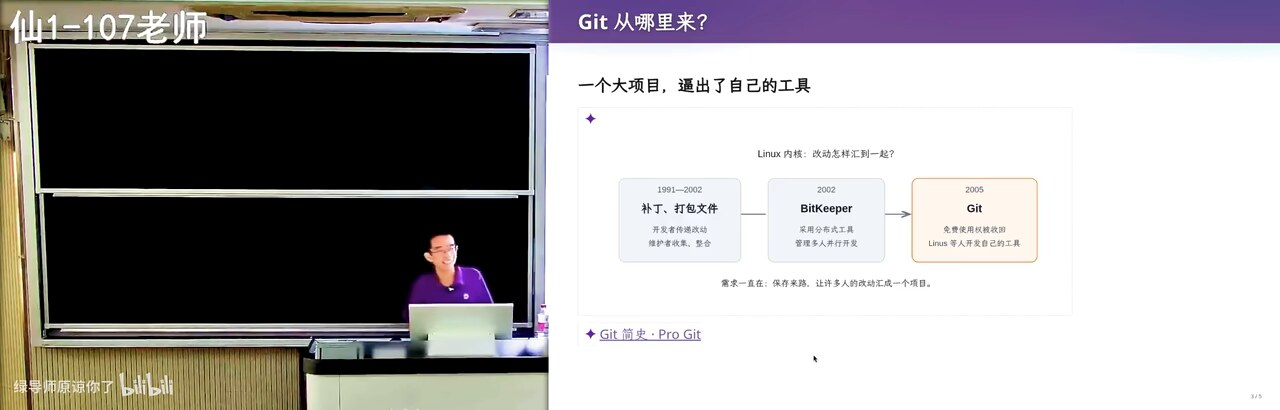
\includegraphics[width=\textwidth]{figures/fig_11_git_history_timeline.jpg}
\caption{Git 简史（ProGit）：1991--2002 邮件补丁 → 2002 BitKeeper → 2005 Git 自研\vtag}
\end{figure}
\srcnote{00:33:15--00:33:29}

\begin{knowledgebox}{延伸阅读}
讲者点名 ProGit 一书；“当然直接让 Agent 看就可以了，不需要再去读了”——书还在，读法变了。
\end{knowledgebox}

\subsection{让概念从已有经验里长出来}

幻灯片把“外推学习”写成三条映射：你知道改错了想撤销 → 项目需要能回去的旧状态；你知道几个文件要配套 → 应当记住项目在同一时刻的样子（快照）；你知道多人会同时修改 → 需要知道各自从哪里出发，才能汇合改动。按这条线，一个大学生从 first principles 推出 Git 的形状是完全可能的——这也是讲者上课“每一句话都和之前有逻辑关联”的原因：这种讲法本身就是数学推理，与 OpenAI“先把数学训好”的信念同构。

\begin{figure}[H]
\centering
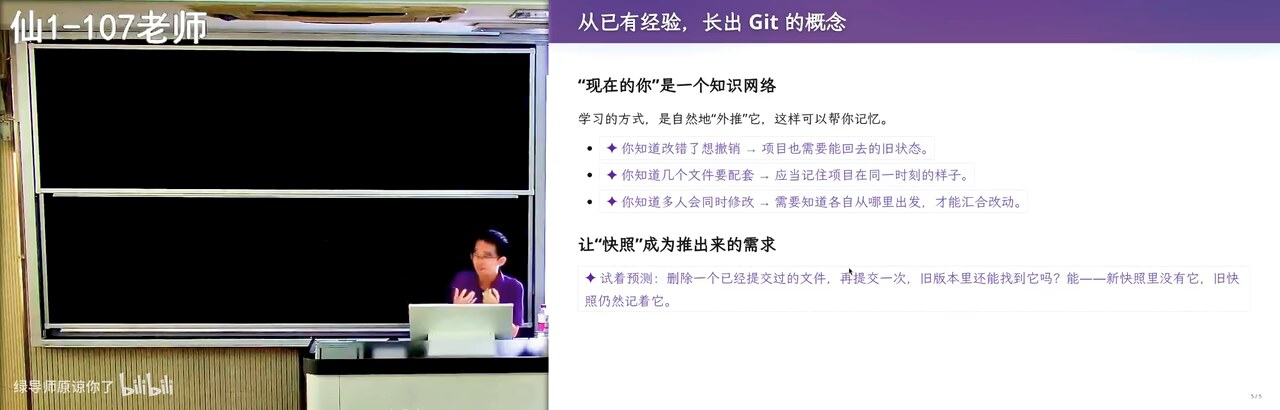
\includegraphics[width=\textwidth]{figures/fig_12_derive_git.jpg}
\caption{从已有经验长出 Git 的概念：撤销、配套快照、汇合改动三条外推线\vtag}
\end{figure}
\srcnote{00:34:15--00:34:29}

\subsection{本章小结}
历史有两条路：存增量与存快照。增量省空间、付回退税；快照共享内部节点后几乎不多花钱，回退一步到位。Linux 项目用十余年试错把后一条路走成了行业标准。接下来的问题自然是：快照具体怎么存？先用起来再说——下一节进入最小工作循环。

\section{最小工作循环：init、add、commit 与一条消息}

\subsection*{本节回答的问题}
Git 的日常最小闭环是什么？“会用”与“符合 best practice”差在哪？

\subsection{init：一切只是一个隐藏目录}

\texttt{git init} 之后目录里多出一个默认不显示的 \texttt{.git}，项目即成为被 Git 版本管理的仓库——“这就是全部了”。从此可以从远端下载、向远端推送，也可以本地记录每一步变化。

\begin{figure}[H]
\centering
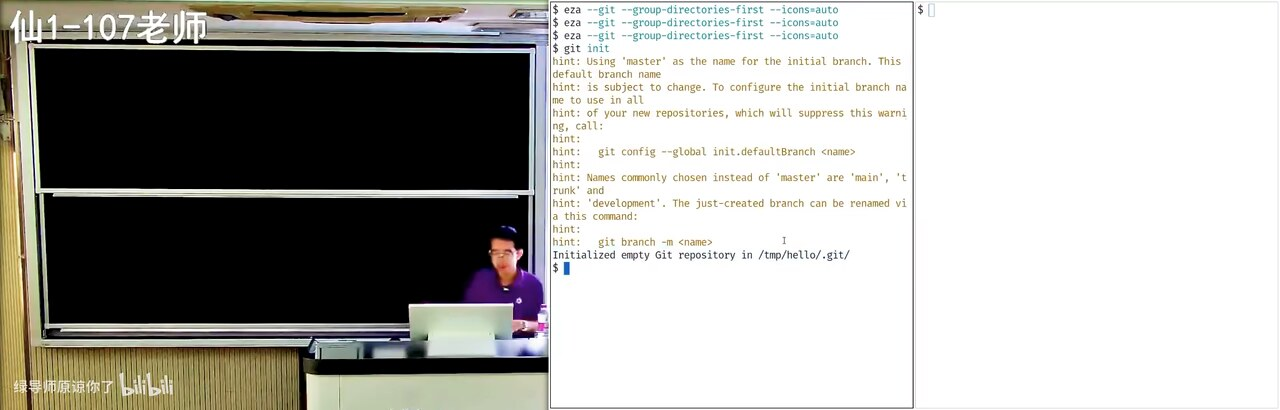
\includegraphics[width=\textwidth]{figures/fig_13_git_init.jpg}
\caption{git init：hint 提示初始分支名 master；仓库的全部物理存在就是 .git 目录\vtag}
\end{figure}
\srcnote{00:35:15--00:35:29}

写一个 \texttt{hello.c}，\texttt{git add hello.c} 进暂存区，\texttt{git status} 会显示工作区状态与下一步提示——Git 的每条输出都是“路牌原则”的执行：在决策点写清可做什么。

\begin{figure}[H]
\centering
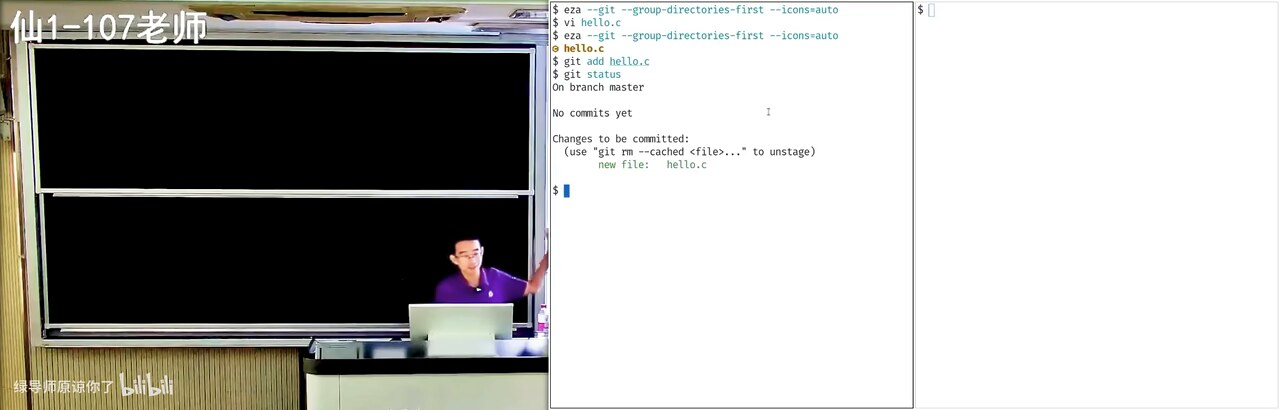
\includegraphics[width=\textwidth]{figures/fig_14_git_add_status.jpg}
\caption{git add 与 git status：工作区（untracked/modified）与暂存区（staged）的双区模型\vtag}
\end{figure}
\srcnote{00:36:15--00:36:29}

\subsection{commit 是“带消息的快照”}

Git 的核心动作是创建项目快照，让人可以在任意时间之间穿梭。“这体现了软件工程的智慧”：不是复制目录改名 v1、v2，而是每做完一件完整的事就提交一次。讲者观察到，很多同学实际上把 Git 当“作业-v1、作业-v2”在用——能跑，但不是长期工程实践中沉淀出的做法。什么时候 add、什么时候 commit、message 怎么写，这些“为什么”不能全交给 AI，需要人自己追问。

\begin{warningbox}{把 Git 当“作业-v1”用}
快照模型的自由很容易诱导成旧习惯：改乱了就整目录另存一份再从头试。讲者观察到不少同学正是这样用 Git——能跑，但它绕开了历史审计：提交不再对应意图，bisect 失去单调前提，冲突定位退化成猜。工具没错，用法把它降级了。
\end{warningbox}

\begin{lstlisting}[language=bash, caption=最小工作循环中与本节演示对应的命令序列]
$ git init                      # 创建仓库（.git）
$ vi hello.c
$ gcc hello.c -o hello          # 编译产物 hello 出现在目录里
$ git add hello.c               # 源码进暂存区
$ git status                    # 查看工作区/暂存区状态
$ git commit -m "feat: add hello world"   # 创建带消息的快照
$ git commit --allow-empty -m "chore: finalize v0.1"  # 无改动的收尾提交
\end{lstlisting}

\subsection{消息是项目的年轮}

虽然 Git 存的是快照，项目本质上仍是从 $V_1$ 经一次次修改走到 $V_R$ 的序列，所以 message 必须描述“改了什么”：一直往下读，就能看见项目怎么发展到现在——修了多少 bug、加了什么需求、经历了什么重构。如果一万个提交都写着 \texttt{I did some cool stuff}，提交历史就成了 slop，这个特性“就不应该存在”。课堂上故意提交了一条这样的垃圾消息，AI 评审一秒钟返回：不太符合 best practice，主要问题在提交信息（可读性为零），其次代码本身也有问题；并建议用祈使句、现在时描述变更动机（例如 \texttt{Fix off-by-one in strlen check}），前缀可参考 Conventional Commits 约定。

\begin{figure}[H]
\centering
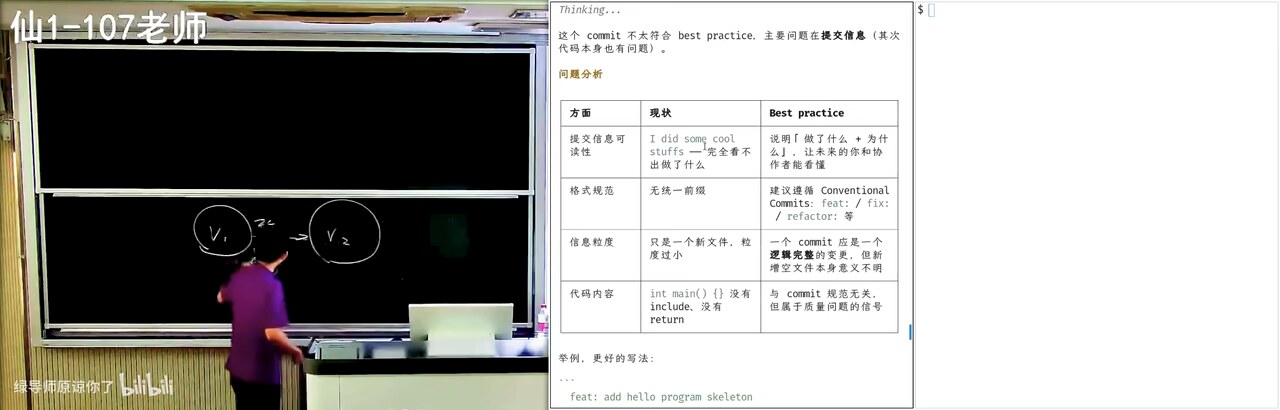
\includegraphics[width=\textwidth]{figures/fig_15_commit_review_ai.jpg}
\caption{AI 评审 I did some cool stuff：主要问题在提交信息，其次代码本身；建议遵循 Conventional Commits\vtag}
\end{figure}
\srcnote{00:40:30--00:40:44}

\subsection{空提交：合法的例外}

没有任何改动时 \texttt{git commit} 会拒绝。但加 \texttt{-\/-allow-empty} 就能强行留一条记录——agent 知道这个知识，人未必。用途有二：无改动时触发 CI；把“修完最后一个 bug”与“发布收尾”拆成两条历史（bug-fix 提交与 finalize 提交分离，tag \texttt{v0.1} 也可完成同样的事）。这是偶尔允许的例外，不能大量制造。

\begin{figure}[H]
\centering
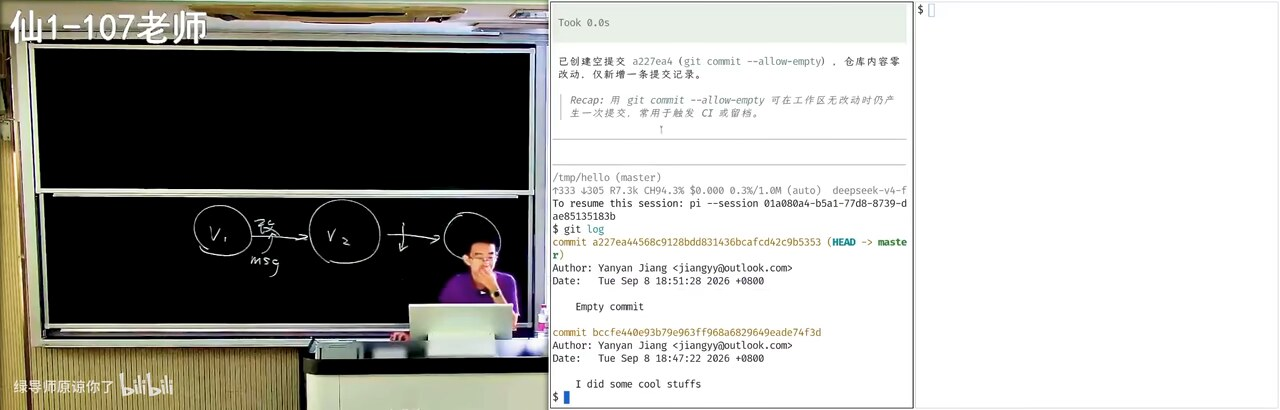
\includegraphics[width=\textwidth]{figures/fig_16_empty_commit.jpg}
\caption{git commit --allow-empty：仓库内容零改动，仅新增提交记录；常用于触发 CI 或留档\vtag}
\end{figure}
\srcnote{00:42:30--00:42:44}

\begin{importantbox}{最小循环的行为准则}
每一次完整改动 → 一次 commit；message 用祈使句写清动机；实验前必先留检查点。模型、测试通过、构建成功是提交的三道门——提交应当是一个完整自洽的快照。
\end{importantbox}

\subsection{本章小结}
命令不过两三样就能跑，水面下的冰山是 best practice，“每一个都是血和泪的教训”。这一节把“提交什么”留给了下一节：仓库应该装什么、又必须挡住什么。

\section{仓库卫生：什么该进，什么该挡}

\subsection*{本节回答的问题}
提交内容与提交历史各自的红线在哪里？

\subsection{编译产物：一个必然的冲突源}

演示故意把 \texttt{hello.c}（2 行改动）与编译产物 \texttt{hello}（15KB 二进制）一起提交，合法但不合格。AI 评审按严重程度排序：第一，提交信息毫无信息量——slop、没说明改了什么；\texttt{Empty commit} 式的消息在“描述操作”而不是“描述内容与原因”；\texttt{I did some cool stuffs} 被直斥为主观废话。第二，提交粒度与内容混杂：编译产物根本不该进版本库，应加入 \texttt{.gitignore}、由构建系统产出。

原因不止“占地方”。每个人的环境不同，build 出的二进制可能带日期、hash 甚至本机指纹——同样的源码，编译结果就是不一样；一万个文件、一百个合作者时，两个不同的 \texttt{hello} 在合并时会产生\emph{二进制冲突}，而二进制没有行级合并的可能（生成图片同理）。仓库防膨胀，防的正是这类必然冲突。

\begin{figure}[H]
\centering
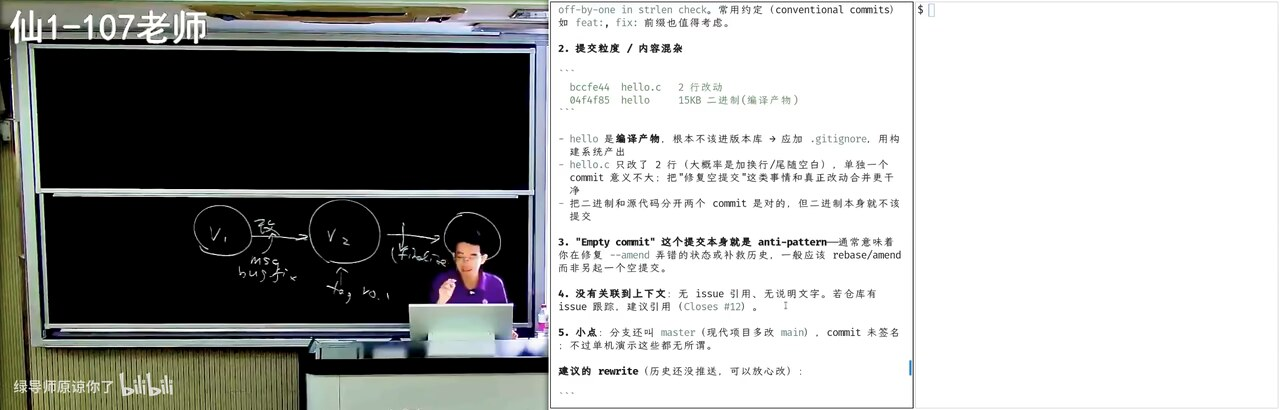
\includegraphics[width=\textwidth]{figures/fig_17_binary_gitignore.jpg}
\caption{按严重程度排序的评审：提交信息毫无信息量居首；15KB 二进制编译产物必须移出、加入 .gitignore\vtag}
\end{figure}
\srcnote{00:47:00--00:47:14}

\subsection{进组以后的高血压时刻}

讲者对研究生新生的四条军规：生成的文件不提交（\texttt{dist/}、\texttt{log}）；个人配置不提交（\texttt{.vscode} 里的个人设置——里面可能写着 C 盘的绝对路径，换台机器就无法复现）；密钥不能提交（审稿时见过好多处于 active 状态的 API key，看到 DeepSeek 的 key 就知道“这应该是一个中国兄弟”）；临时文件不提交（macOS Finder 逛一逛目录就留下的 \.DS\_Store，以点开头、默认隐藏，\texttt{ls} 甚至还给它画了个苹果图标，\texttt{git add .} 一锅端时最容易误入）。

规则是活的，判断标准是用途而不是目录名：\texttt{package-lock.json}、为免装工具链而生成的 header，恰恰应当提交——它们让别的环境不装依赖也能构建；团队共享、可移植的配置可以提交。还有一条常被忽略的边界：\texttt{.gitignore} 只挡未跟踪文件，\emph{不会}让已被跟踪的文件自动退出版本管理——“忽略不等于遗忘”。

\begin{figure}[H]
\centering
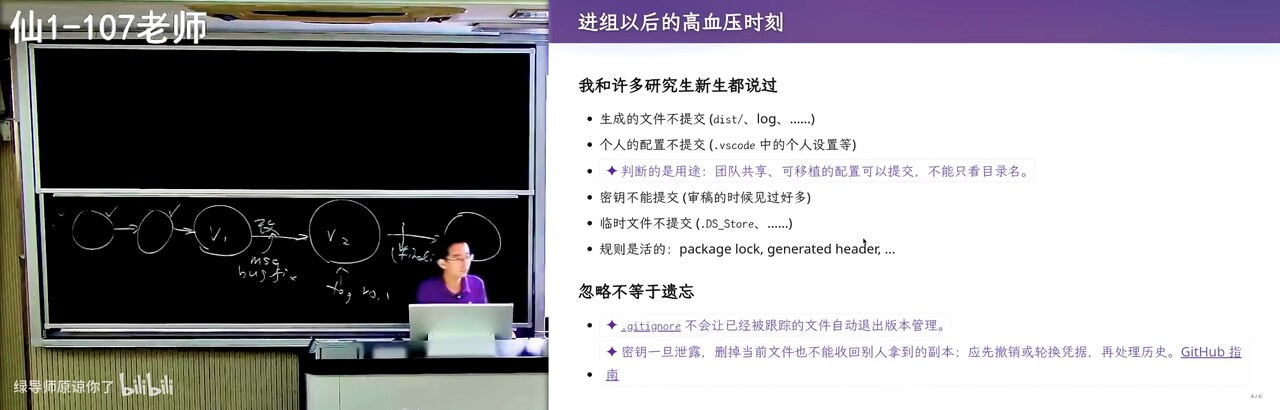
\includegraphics[width=\textwidth]{figures/fig_22_hypertension_moment.jpg}
\caption{进组高血压时刻：生成文件、个人配置、密钥、.DS\_Store；规则是活的，看用途不看目录名\vtag}
\end{figure}
\srcnote{00:55:15--00:55:29}

\begin{warningbox}{git add . 的双面性}
点文件默认会被 \texttt{git add .} 收进来，因为 \texttt{.github/workflows} 这类约定本就该跟踪；同一机制也让 \.DS\_Store 混入。先配 ignore 清单再图省事，或者让工具逐文件审查（见下一节）。
\end{warningbox}

\subsection{整理历史：只有在没人依赖时才安全}

演示让 agent 把这段混乱历史整理掉。它先检查了一个关键事实：仓库历史\emph{没有 remote}——没有任何协作者持有旧历史，重写才安全；“如果别人也持有，那就是一个比较糟糕的事情了”。随后按对照表执行：

\begin{center}
\small
\begin{tabular}{lll}
\toprule
原问题 & 处理 & 依据 \\
\midrule
slop 提交信息 & 改写为 feat:/chore: 前缀祈使句 & 消息面向未来的读者 \\
空提交 & 重写时剔除 & 例外不留入主干 \\
二进制 hello 入库 & 移出历史并加 \texttt{.gitignore}，磁盘文件保留 & 新历史从未包含它，重写无副作用 \\
分支名 \texttt{master} & 改名 \texttt{main} & 社区约定迁移 \\
\bottomrule
\end{tabular}
\end{center}

验证方式同样讲清：\texttt{git status} 干净、\texttt{git check-ignore} 确认 hello 已被忽略。整理后 agent 甚至顺手发现历史里可以塞更多机关——例如 message 里写 \texttt{fixed \#3}，GitHub 会自动关闭对应 issue。

\begin{figure}[H]
\centering
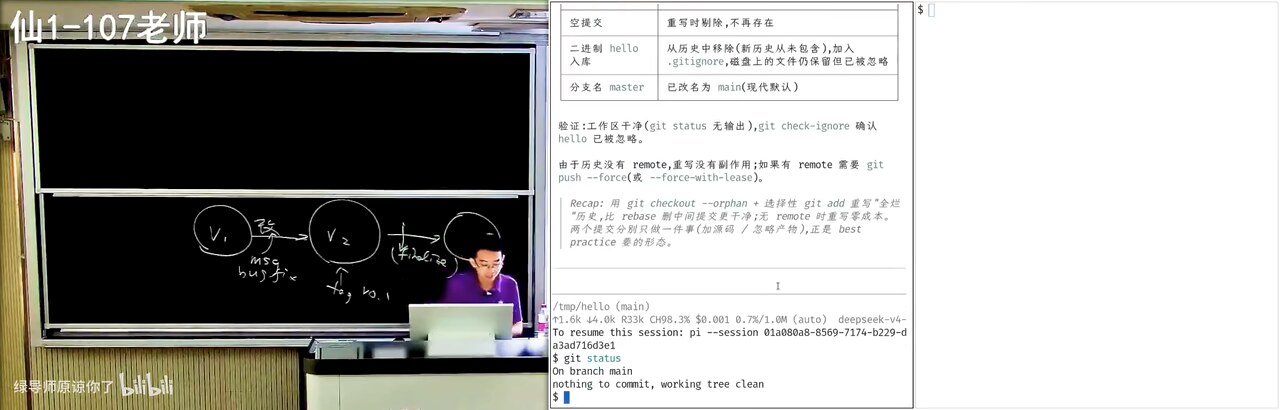
\includegraphics[width=\textwidth]{figures/fig_18_rewrite_history.jpg}
\caption{agent 重写历史的处理清单：先确认无 remote，再逐条改写；验证以 git status / check-ignore 为准\vtag}
\end{figure}
\srcnote{00:49:15--00:49:29}

\subsection{本章小结}
“提交什么”看内容用途，“改历史”看有没有人依赖。两条红线都源于同一件事：仓库是给人、也给未来的你和协作者读的历史书。可是靠人肉逐条检查太累，讲者把检查外包给了一个文件——下一节。

\section{可审计性：让历史能回答“为什么”}

\subsection*{本节回答的问题}
如何在不增长人肉注意力的前提下，持续产出符合 best practice 的提交？bisect 与 blame 怎样把历史变成可搜索的证据链？

\subsection{AGENTS.md：让 agent 先检查再操作}

项目的 \texttt{AGENTS.md} 里只加一条约定：“在做任何 git 操作之前，都逐个文件检查变化，并为我（新手）解释是否符合 best practice、为什么、以及相关的概念。”此后每次提交前，agent 都会先看一眼再放行或拦下。

\begin{figure}[H]
\centering
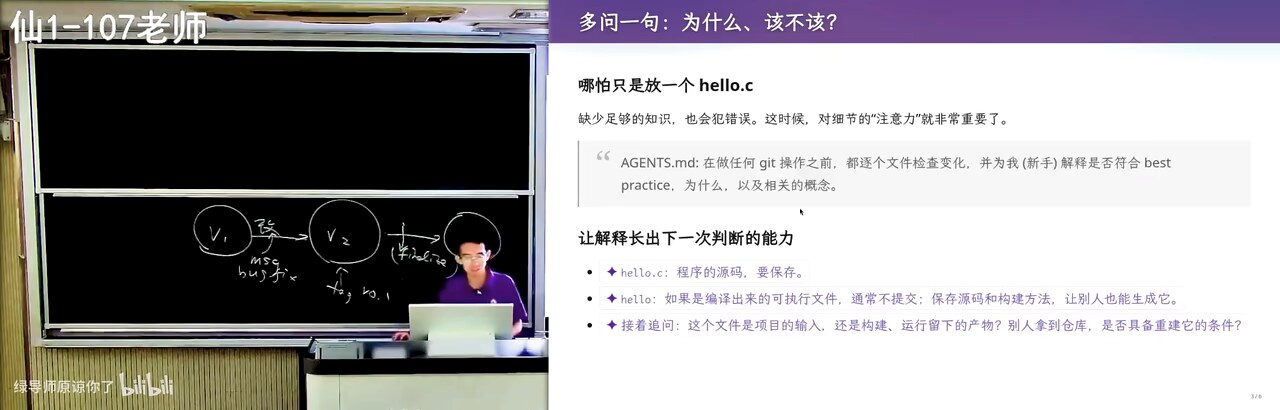
\includegraphics[width=\textwidth]{figures/fig_19_agents_md.jpg}
\caption{“多问一句：为什么、该不该？”——AGENTS.md 把检查与解释固化为提交前动作\vtag}
\end{figure}
\srcnote{00:50:45--00:50:59}

\subsection{提交必须编译得过去}

一次故意提交不能编译的代码（在 \texttt{hello.c} 里加了一行裸的 \texttt{a}），agent 逐文件给出结论：\texttt{'a' undeclared}、缺分号，当前不建议直接提交，并把代码修好。它给出的理由被讲者盛赞“我上课急就时我是想不到他的”：\textbf{Git 提交应当是一个完整自洽的快照，提交编译不过的代码等于让仓库处于坏状态}。若有人要 \texttt{git bisect}，坏快照会直接毁掉二分的前提。

\begin{figure}[H]
\centering
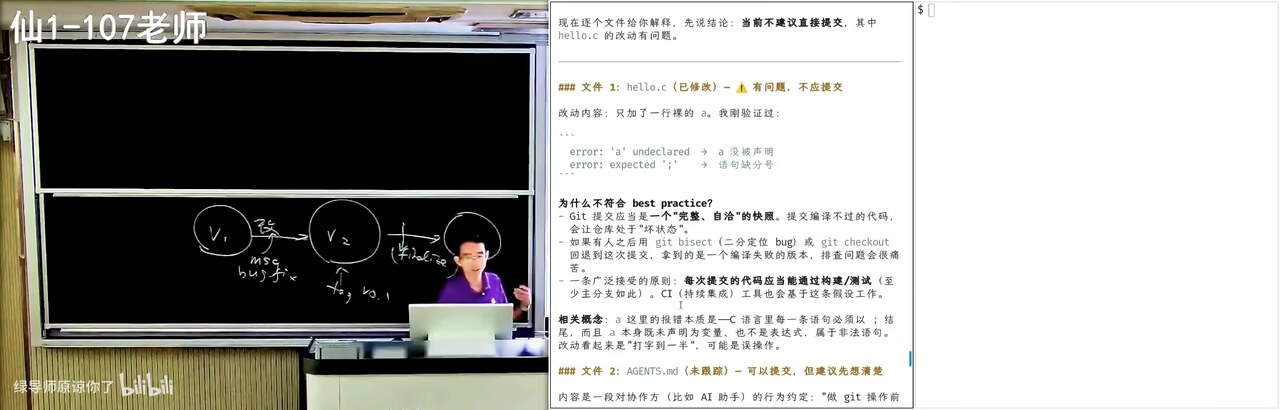
\includegraphics[width=\textwidth]{figures/fig_20_file_review.jpg}
\caption{agent 逐文件审查：先验证 error: 'a' undeclared、缺分号，再判定不应提交并解释原因\vtag}
\end{figure}
\srcnote{00:52:00--00:52:14}

\subsection{bisect：历史是一个前 0 后 1 的数组}

把提交历史想成一个数组：当前版本有 bug，但 bug 未必由这次改动引入；只要有一个能判定 bug 是否存在的测试，就可以对整个历史做二分——某个提交之前都正常，之后都不正常。形式化地：

\begin{equation}
i^{*}=\min\{\, i : f(V_i)=1 \,\},\qquad f(V_i)\in\{0,1\},\quad f \text{ 单调非降}
\end{equation}
式中 \(V_i\) 是第 \(i\) 次提交的状态，\(f(V_i)\) 为测试在该状态的结果（0 通过、1 失败），单调性由“bug 一旦被引入就不会自行消失”保证；二分把 \(O(n)\) 次构建降为 \(O(\log n)\) 次。

\begin{knowledgebox}{先学数学，再学一切？}
讲者把 OpenAI 的路线与本课方法视为同构：数学拥有全球公认的推理系统，是最可靠的 grounding；训好数学后，其他能力可以借强化学习外推。对应到学习法上，就是“每一句话都与之前有逻辑关联”——像做数学一样把工程概念逐个推出来，而不是逐个背下来。这是讲者的信念式解读，业界对 AGI 路线并无共识。
\end{knowledgebox}

知道错在哪之后，\texttt{git blame} 回答另一问：每一行代码是哪一次提交、由谁改的——即使历史完全线性，也能做很多有趣的事。幻灯片边角的帮助文本里能看到配套开关（如 \texttt{-\/-ignore-rev} 在 blame 时忽略纯格式化提交）。

\begin{figure}[H]
\centering
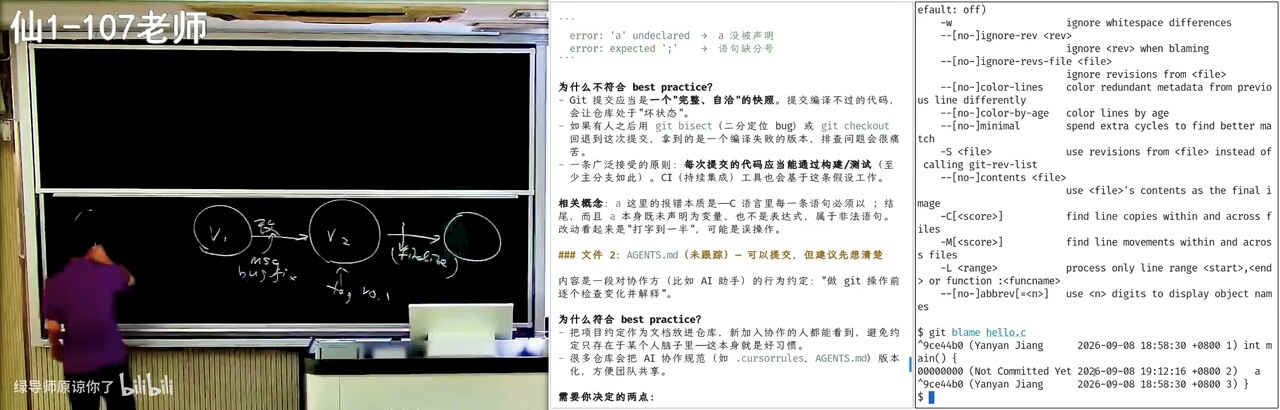
\includegraphics[width=\textwidth]{figures/fig_21_bisect_blame_help.jpg}
\caption{bisect/blame 相关帮助文本：--ignore-rev、--w 忽略空白差异等选项是审计工具的人性化边界\vtag}
\end{figure}
\srcnote{00:53:15--00:53:29}

\subsection{被大模型“杀死”的 best practice 检查器}

一段讲者自述的研究史：软件工程研究的一个标准题目，是检查 Git 项目是否满足 best practice——几十条规则、一堆 warning、一个提交前拦截小工具（讲者实验室就有对应产物）。如今“所有这些东西都被大模型杀死了”，因为大模型可以如此耐心地逐文件检查，还会“给你一个 emoji，让你开心一下”。同样被消解的还有高学压时刻：导师把学生叫到办公室批评，无论情绪多正常，学生总有压力；AI 不会让你有这种压力。

\subsection{隐形的知识：大写还是小写？}

一个真实项目的两难：给 check 规则命名，\texttt{[TYPO-CHECK]} 还是 \texttt{[typo-check]}？讲者的直觉是全大写更好，但“不是极强，不太说得出原因”。先想一想：方括号里的字符，是一句话的一部分，还是一个\emph{可以被引用的规则名字}？追问 AI 后得到带引用出处的解释。学习生活中无穷多这样的小两难，每个都多问一句，就积累了大量暗知识——“你们一定会 become a lot better person”。

\begin{figure}[H]
\centering

\includegraphics[width=\textwidth]{figures/fig_23_case_choice.jpg}
\caption{真实项目中的命名两难：[TYPO-CHECK] vs [typo-check]，直觉值得追问\vtag}
\end{figure}
\srcnote{00:59:30--00:59:44}

\begin{importantbox}{把“多问一句”制度化}
AGENTS.md 式约定 = 个人注意力的外部化。它把“这符合 best practice 吗”从每次现场想，变成提交前自动发生的一次对话——工具替你保留了注意力，你负责保留判断。
\end{importantbox}

\subsection{本章小结}
审计链条 = 小步提交（可 bisect）+ 每行溯源（blame）+ 坏快照零容忍。这些机制要求历史“拆得好”；而历史拆得好不好，取决于下一条 best practice 合集里的日常纪律。

\section{Best Practice 合集：让错误可恢复，让协作可预期}

\subsection*{本节回答的问题}
把散落的 best practice 归拢起来：哪些规则保证自己摔了能爬起来，哪些保证与别人一起走不互相绊倒？

\subsection{给自己留退路}

\begin{warningbox}{提交不等于备份：未提交文件的边界}
“提交了就安全”只对已提交的内容成立：远端 clone 不包含你工作区与暂存区里未提交的文件；只 commit 不 push，硬盘物理损坏依然是全损。完整链条是改动→提交→推送，一环不落；反过来，误操作后先停止写入、保护现场，再用 \texttt{reflog} 找回。
\end{warningbox}

幻灯片口诀：Commit often, perfect later, publish once。及时 commit 的深层理由不是“保存进度”，而是复杂性放大错误：小项目一次提交两三千行无妨；一旦项目有错综复杂的关系，一个大 commit 可能同时破坏多处、引入多个 bug，后面一百个修复都挂在这一个一万行的 commit 上——修不过来，也说不清修没修好。小提交则“冤有头债有主”，bug 与 fix 可以配对，历史获得审计能力。物理风险同理：改了就提交、提交就 push，等于给自己留了一份互联网上的备份；本地未推送的修改救不了损坏的硬盘，而\emph{远端 clone 也不包含你未提交的文件}。误操作后先保护现场再查 \texttt{reflog}——reflog 是 Git 给自己的后悔药。

\begin{figure}[H]
\centering
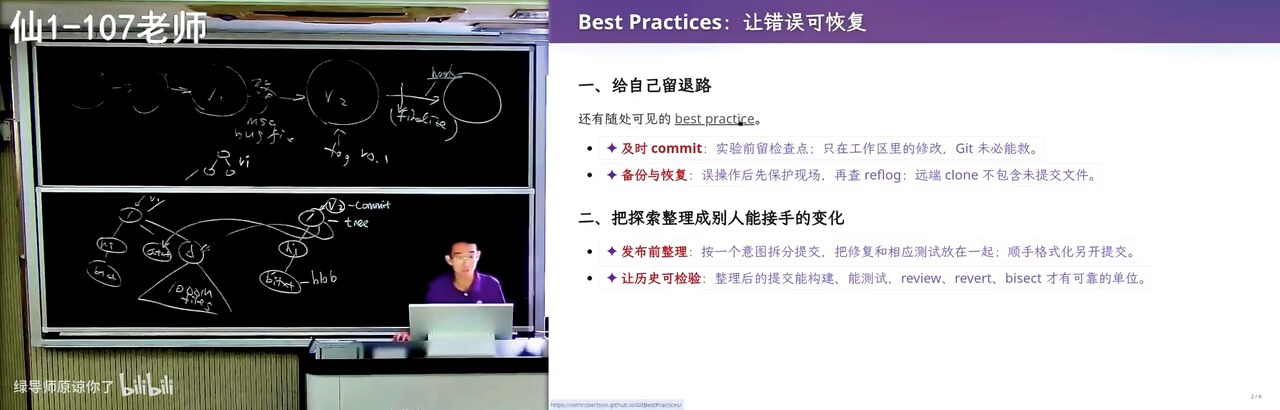
\includegraphics[width=\textwidth]{figures/fig_35_rollback_reflog.jpg}
\caption{Best Practices·让错误可恢复：及时 commit 留检查点；备份与恢复先护现场再查 reflog\vtag}
\end{figure}
\srcnote{01:29:30--01:29:44}

\subsection{约定要能写下来：Conventional Commits 与一个空格}

AI 生成的提交信息已经开始“自由发挥”：中英混排、有时无 scope。但格式确有标准——Conventional Commits 规范原文要求提交必须以 type 前缀（feat、fix 等名词）+ 冒号 + 空格开头；它解释引入约定的动机：跨项目边界制造一种共同语言，让 debug 更容易。同一逻辑的极端小样：Markdown 文档里中英文之间加空格——“你好，这是hello.c”这种忽此忽彼的排版让人“浑身难受”；一致比美观重要。讲者顺带自省：代码要以同样的方式排版，文档同理；虽然“AI 时代好像也不重要，AI 都会帮你记得”。

\begin{figure}[H]
\centering
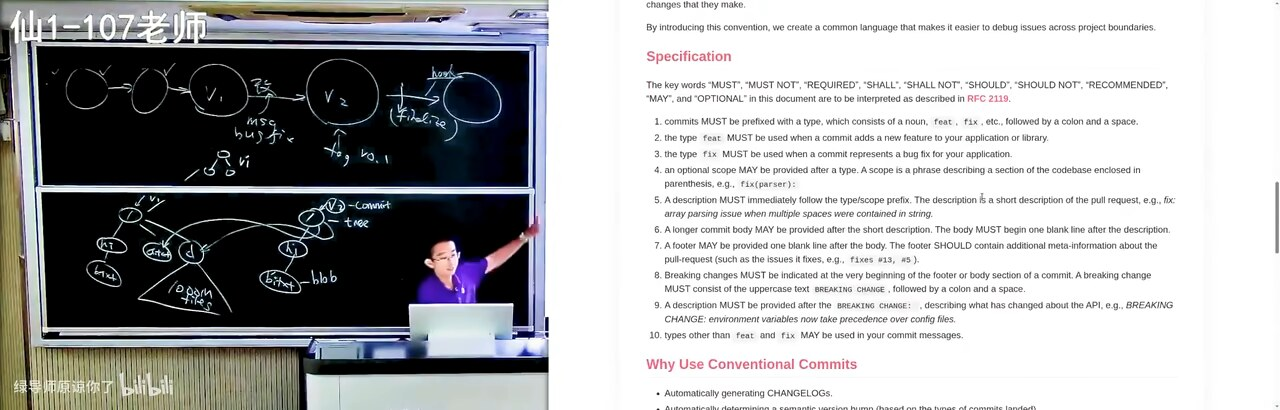
\includegraphics[width=\textwidth]{figures/fig_33_conventional_commits.jpg}
\caption{Conventional Commits 规范：type 前缀 + 冒号 + 空格是硬性规定，目的是跨项目的共同语言\vtag}
\end{figure}
\srcnote{01:27:30--01:27:44}

\begin{figure}[H]
\centering
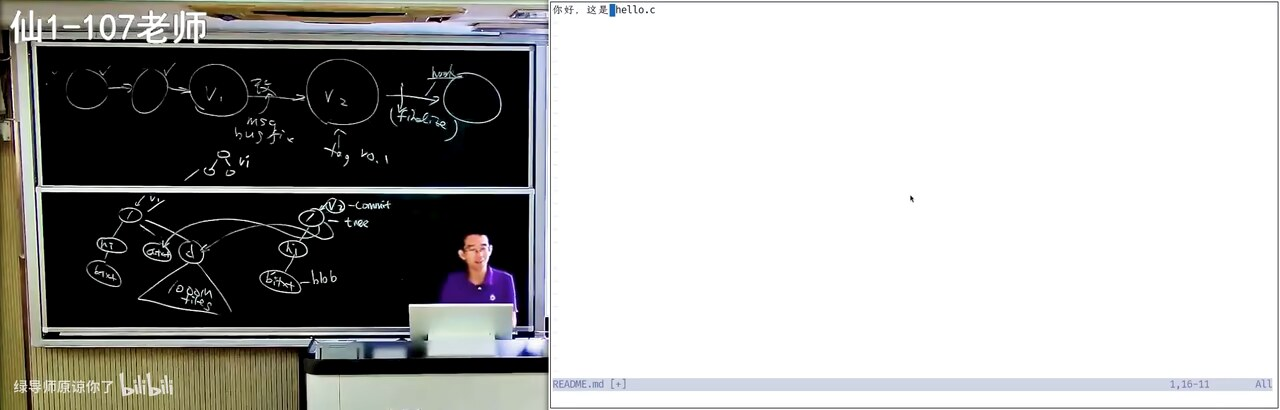
\includegraphics[width=\textwidth]{figures/fig_34_cjk_spacing.jpg}
\caption{一致性约定演示：同一段文字中英文空格忽有忽无，比全都不加更刺眼\vtag}
\end{figure}
\srcnote{01:28:15--01:28:29}

\subsection{协作可预期：历史、分支与守门机制}

不擅自改写\emph{别人依赖的}历史——改写会把整理成本转嫁给协作者，修错通常追加提交；分支与发布流程要有约定：谁合并、如何回移补丁、何时打 tag。约定要有执行机制：本地用 pre-commit hook 尽早反馈，服务端用 CI 守住合入条件，同步上游后重新测试组合结果。hook 是通用机制：函数调用完成时可以挂一个动作，agent 也能挂——讲者演示了一个“agent 需要输入时叮一声”的全局 hook，各主流 agent（Claude Code、Codex、Cursor 等）都支持同类配置。

有些项目进一步要求 linear history：合并可以用双 parent 的 merge commit，但如今流行靠 rebase 把历史强行拉直。理由在 AI 时代更实际：历史线性、拆分得好，定位一次修改更容易，AI 维护项目时更省 token、有些文件可以直接不读；cherry-pick 与 blame 也更友好。讲者提醒这并非全是好处——它是当前维护成本下的权衡，“在无限大能力的模型到来之前，这条法则成立”。

\begin{figure}[H]
\centering
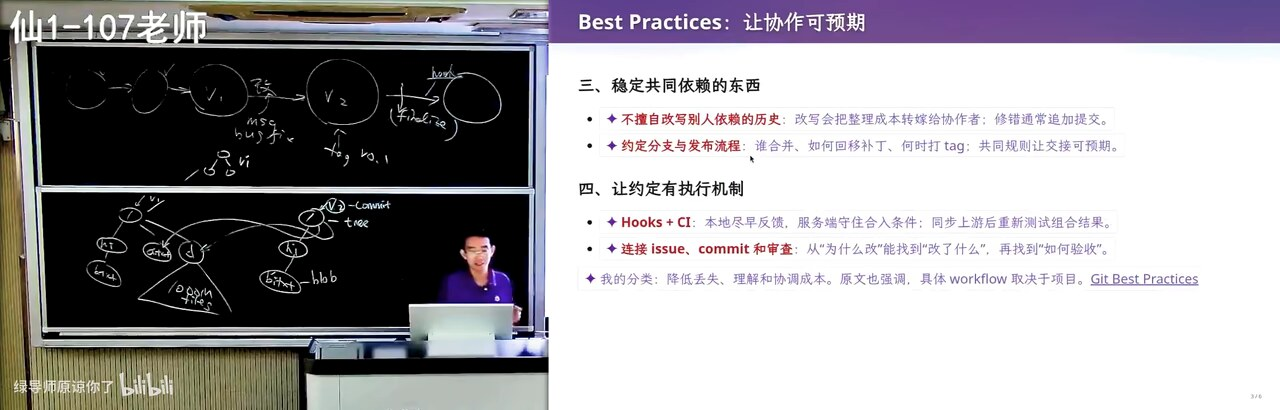
\includegraphics[width=\textwidth]{figures/fig_36_hooks_ci_collab.jpg}
\caption{让协作可预期：不重写他人依赖的历史；Hooks 本地反馈 + CI 守合入条件\vtag}
\end{figure}
\srcnote{01:31:15--01:31:29}

\subsection{Git 之外：gh 与 glab}

issue、PR、评论这些对象不随 Git tree 持久化——它们住在平台上。GitHub 太流行，于是有了把平台操作命令行化的 gh（GitLab 对应 glab）：fetch 指派给你的 issue、发起 PR、查 CI 状态。agent 装了 gh 之后可以直接接一条长任务：读 issue、开发、小步提交、开 PR——这正是“可以审计的提交”在流水线上的价值。agent 探测到未装 gh 时会“回退到古法编程”继续裸写 git 命令。

\begin{figure}[H]
\centering
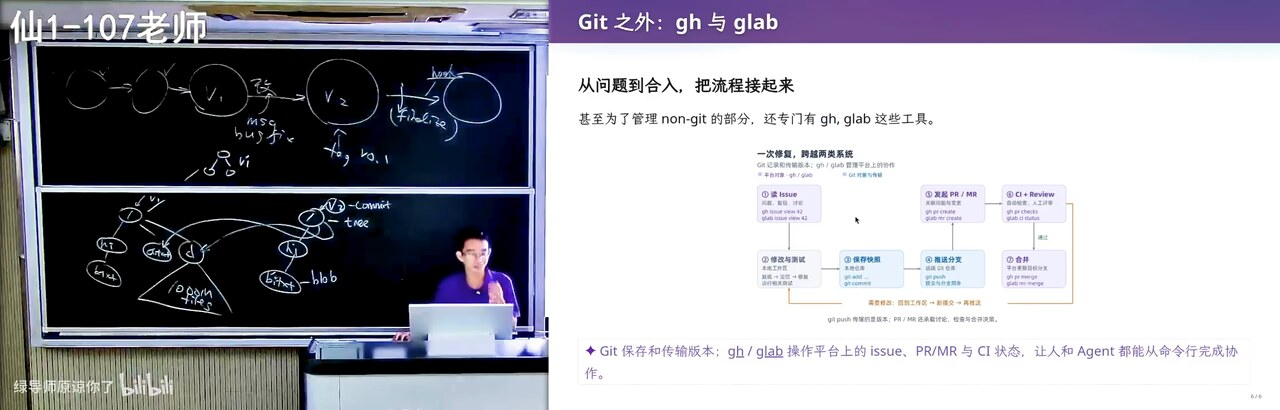
\includegraphics[width=\textwidth]{figures/fig_37_gh_glab.jpg}
\caption{一次修复跨越两类系统：issue/PR 由 gh / glab 管理，代码版本由 Git 管理\vtag}
\end{figure}
\srcnote{01:32:30--01:32:44}

\begin{lstlisting}[language=bash, caption=幻灯片中的 gh / glab 对应命令（一次“读 issue → 发 PR → 查 CI”的闭环）]
# GitHub CLI
$ gh issue view 42
$ gh pr create
$ gh pr checks
# GitLab CLI
$ glab issue view 42
$ glab mr create
\end{lstlisting}

\subsection{本章小结}
这一节的每条规则都能被一句话推出：历史是审计对象。留退路保证审计可回滚，写约定保证审计可读，hook+CI 保证审计不被绕过，gh/glab 把审计范围从代码扩展到协作对象。

\section{Git 的内核：一个持久化数据结构}

\subsection*{本节回答的问题}
快照模型要“秒回任意版本”，空间上为什么不会爆炸？分支、合并、冲突在磁盘上到底是什么？

\subsection{快照只复制“到根的路径”}

讲者给 Git 的定义只有一句：Git 是一个\textbf{持久化的数据结构}，持久化的是目录树。项目是一棵大树：根下若干文件与子目录。创建 V2 时不需要复制整棵树——改动的只有 \texttt{b.txt}，那就新建一个 \texttt{b.txt} 的新版本，并把\emph{它到根的路径}上的节点各复制一份；未动的 \texttt{a.txt}、子目录 \texttt{d/} 用指针继续指向旧节点。目录树天然浅（没人建一千层目录，渐进式披露也反对巨深目录），每层索引分支是指数级的，于是：

\begin{equation}
\bigl|\text{new}(V_1 \to V_2)\bigr| \;=\; \bigl|\text{changed files}\bigr| \;+\; O(\text{depth}) \;\ll\; |\text{project files}|
\end{equation}
式中 \(\text{new}(\cdot)\) 为新版快照新增的对象数，\(\text{depth}\) 为改动文件在目录树中的深度，根到叶路径上的每个目录节点新建一个、只改指针。一百万个文件的项目，改动几个文件时新增对象仍以“个”计——这就是“快照几乎不多花钱”的机制证明。

\subsection{磁盘上的三件套：blob、tree、commit}

\texttt{.git} 里的 objects 就是带 hash 索引的普通文件，三种节点各一种对象：blob 是字节序列，tree 是“权限 + 名字 + 指针”的目录条目，commit 记录快照根 tree、作者与消息。整个数据结构只朝一个方向生长。为了验证“老师说的真有吗”，讲者用一个实时读取真实仓库的可视化工具打开了仓库（细节见 §10.5）：空 \texttt{hello.c} 的内容 blob 压缩后 31 字节、zlib 解压出 23 字节——小文件压缩反而亏本；可执行文件 \texttt{hello} 的 blob 以 7f 打头（ELF 头）；tree object 52 字节解压出 43 字节，明文形如 \texttt{644 blob <hash>\ \ \ \ hello.c}：mode 644 是普通文件、755 是可执行的 \texttt{hello}，后接名字与指向 blob 的指针。

\begin{figure}[H]
\centering
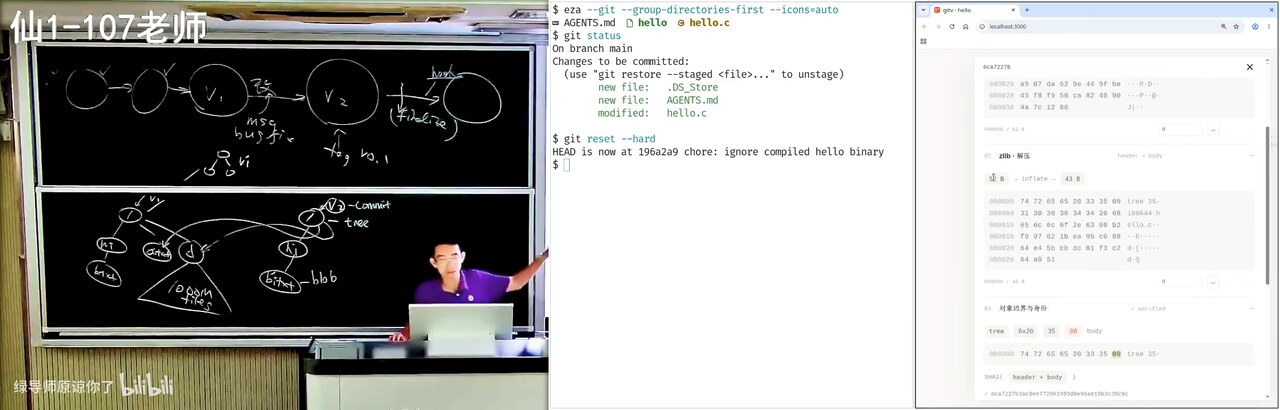
\includegraphics[width=\textwidth]{figures/fig_26_gitv_visualizer.jpg}
\caption{实时可视化 main 分支：commit → tree → blob 的引用关系全部来自磁盘原始字节\vtag}
\end{figure}
\srcnote{01:13:00--01:13:14}

\begin{importantbox}{三件套一句话}
blob 存内容，tree 存目录，commit 存“某一刻的整棵树 + 来路”。快照 = 一个 commit 对象；分支 = 一个指针；历史 = 有向无环图。
\end{importantbox}

\subsection{分支是文件，HEAD 是指针的指针}

在可视化工具里创建两个分支，动画立刻说清本质：所谓分支就是一个叫 ref 的小文件，内容是它指向的 commit 的 hash；HEAD 是指向指针的指针。分支 A 把 \texttt{hello.c} 首行改成 \texttt{int main(void)}（提交 \texttt{94d2b56}），分支 B 改成带命令行参数的签名（提交 \texttt{27e7fd3}）——两处修改重叠在同一行，\texttt{git merge} 时必然冲突。这不是实现瑕疵，而是“两个意图撞车”的最小模型，课堂上让两名同学各重构一次就会进入同样状态。

\begin{figure}[H]
\centering
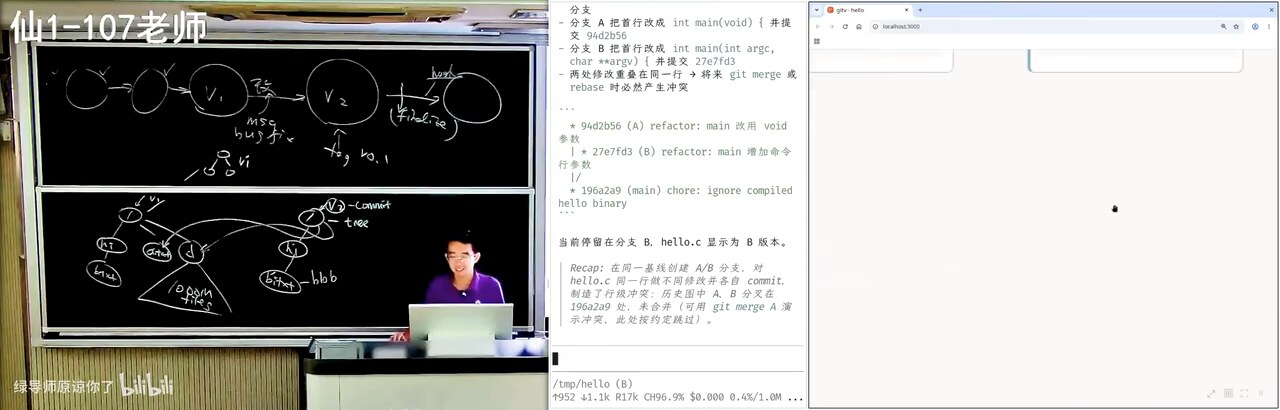
\includegraphics[width=\textwidth]{figures/fig_27_branch_ab_conflict.jpg}
\caption{分支 A/B 修改同一行：两个 commit 各自合法，合并时冲突已在写下的那一刻注定\vtag}
\end{figure}
\srcnote{01:15:00--01:15:14}

\subsection{合并的现场与残局}

把 A 拉向 B 触发冲突后，可视化揭示 Git 悄悄留了\emph{三个版本}：base（共同祖先的该文件）、ours、theirs；工作区里给你看的则是带 \texttt{<<<<<<<} 标记的文件。解决后产生的 merge commit 有两个 parent，作者、树指向解好的版本，指向关系被完整保留——冲突不是历史的伤疤，而是被记录的一次决策。

\begin{figure}[H]
\centering
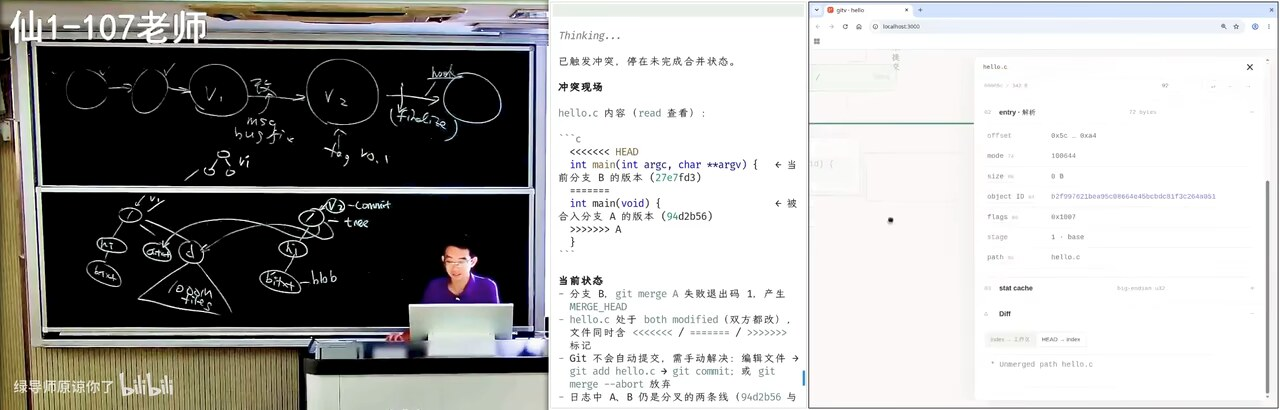
\includegraphics[width=\textwidth]{figures/fig_28_conflict_three_versions.jpg}
\caption{冲突现场透视：Git 内部保存 base / ours / theirs 三份文件，merge commit 带两个 parent\vtag}
\end{figure}
\srcnote{01:17:00--01:17:14}

\subsection{从模拟动画到 vibe-code 的现场可视化}

讲者称 learn git branching 是“古法编程的巅峰之作之一”：以动画模拟 git 命令的教学站。但它毕竟是\emph{模拟}——建了一个 Git 的模型在演示。今天可以直接 vibe-code 出读真实仓库的工具：给 GPT-6 的提示词要求“实现一个 Git 可视化命令行工具，把一个真实 Git repo 的主要概念彻底完整地可视化；展示任何对象前，都从文件系统的真实字节出发，展示一步一步如何解析；持续监听仓库变化，用动画展示变化”。one-shot 直出带若干视觉 slop（讲者原话“视觉效果不完美是因为我没有调”），但对象解析完全真实。这条“告别古法学习”路线的注脚是计算机科学定律：你想要的东西就一定有人做过；而人类视觉系统高效，软件可视化却几十年进展缓慢——直到一句话能生成工具为止。

\begin{figure}[H]
\centering

\includegraphics[width=\textwidth]{figures/fig_24_no_old_learning.jpg}
\caption{告别古法学习：计算机科学定律与“软件可视化几十年进展缓慢，忽然所有问题都解决了”\vtag}
\end{figure}
\srcnote{01:08:00--01:08:14}

\begin{figure}[H]
\centering
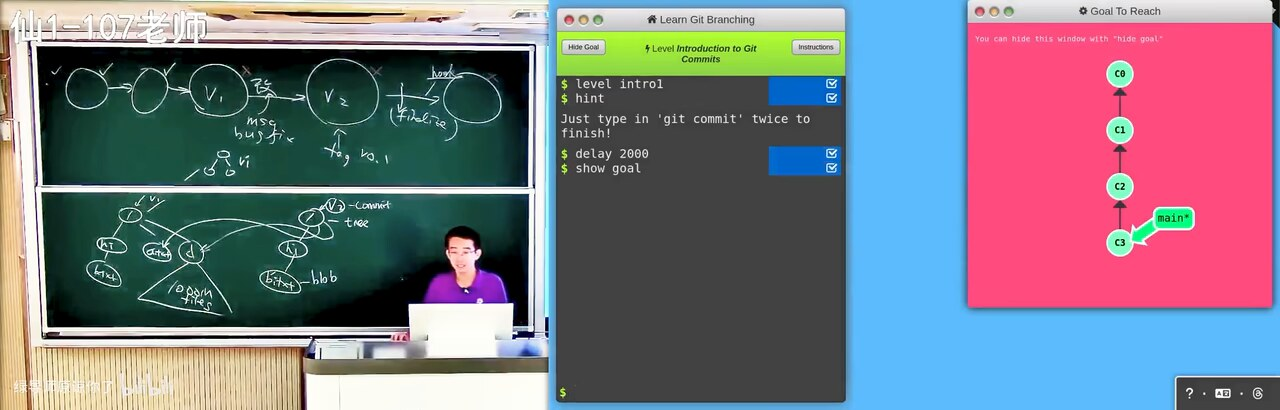
\includegraphics[width=\textwidth]{figures/fig_25_learn_git_branching.jpg}
\caption{Learn Git Branching：以模拟动画演练 commit/branch/merge 的经典教学站\vtag}
\end{figure}
\srcnote{01:08:45--01:08:59}

\subsection{本章小结}
Git 的“魔法”到此全部还原：快照靠共享节点便宜下来，分支只是文件，合并是带两个 parent 的 commit，冲突是三个版本加一堆标记。数据结构讲完，讲者用一组现做工具演示这套知识怎么“被看见”——也是他主张的学法本身。

\section{一句话生成的教学工具：vibe-coding 作为学习方法}

\subsection*{本节回答的问题}
当“做出一个好用的教学演示”不再有成本，这类工具还剩下什么价值？学习者的稀缺品质是什么？

\subsection{从伯克利的 IDE 到自己的 Playground}

UC Berkeley 的 CS61A 用 code.cs61a.org 教 Python：浏览器里一个功能完整的 IDE，能运行、能交作业。讲者团队因为要给三四年级小朋友开 Python 启蒙课，“被迫 vibe-code”了一个类似物：既能当网页应用，也能像 VSCode 一样打包成双击即开的 exe；架构由讲者“稍微把了一下关”，其余全是 AI 直出，代码质量不再管控——“这些 slop 都是我直接让 AI 一句话生成的”。

\begin{figure}[H]
\centering
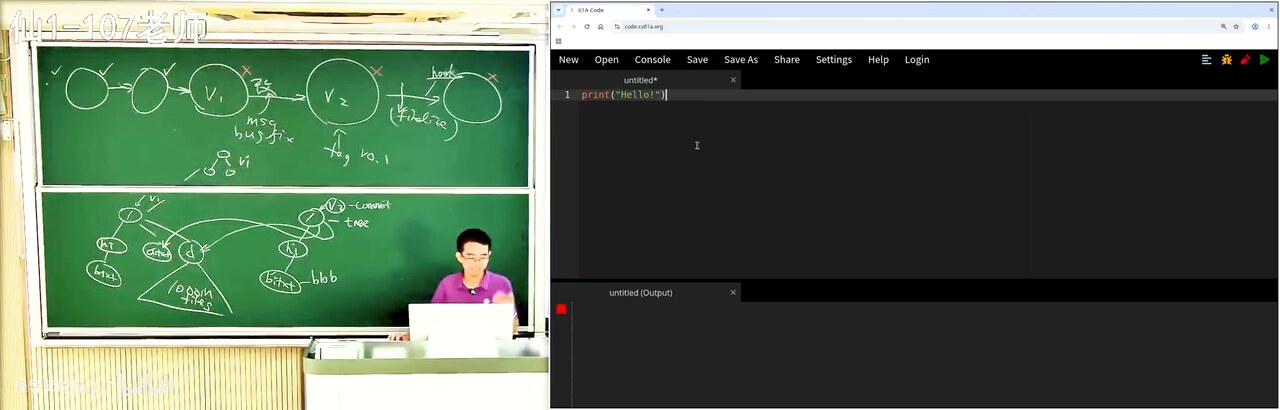
\includegraphics[width=\textwidth]{figures/fig_29_cs61a_ide.jpg}
\caption{code.cs61a.org：浏览器内完整 Python IDE 的官方先例\vtag}
\end{figure}
\srcnote{01:19:00--01:19:14}

第一节课的任务是让小朋友觉得 Python 好玩：把一个 Unicode 字符块编码成整数再 decode 回来；\texttt{hello * 10} 打印十份。随后是可交互的汉诺塔：递归之前先告诉你应该怎么移动，时间轴前后拖动、动画真实移动。再往后是体素世界 Pico World：几行三重循环 \texttt{drop(x, y, "metal")} 就搭出一个可以调试、可以回放的 3D 世界，坐标轴第一版不对，“我还骂了一下 AI”，改后前后拖动的动画平滑。用讲者的话说，快乐源泉没变——二重循环打三角形就能开心，如今是能创造一整个世界。他还验证过用 DeepSeek 等便宜的国产模型编译这类可视化程序，已经达到完全可用的状态。

\begin{figure}[H]
\centering
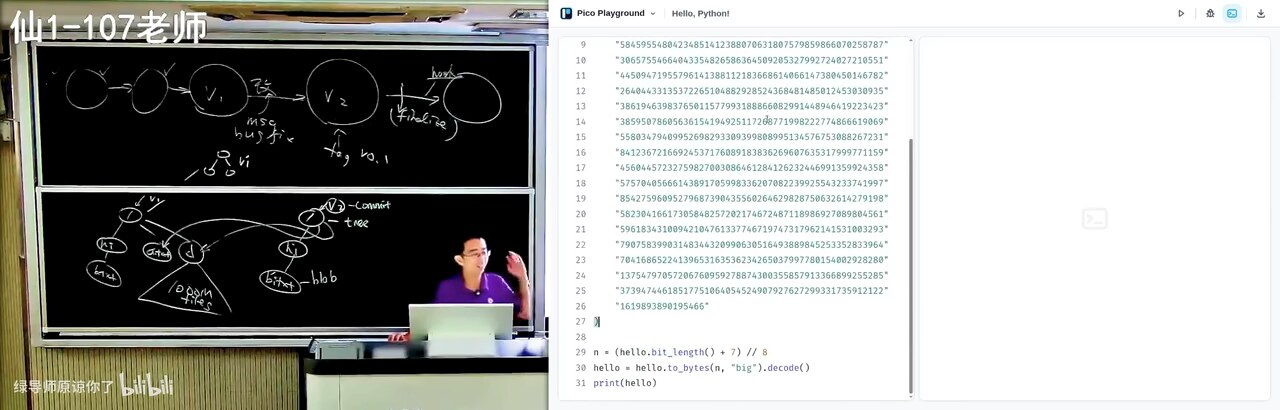
\includegraphics[width=\textwidth]{figures/fig_30_pico_hello_python.jpg}
\caption{Pico Playground 第一课：Unicode 字符 $\leftrightarrow$  整数互转，hello * 10 的视觉惊喜\vtag}
\end{figure}
\srcnote{01:21:00--01:21:14}

\begin{figure}[H]
\centering
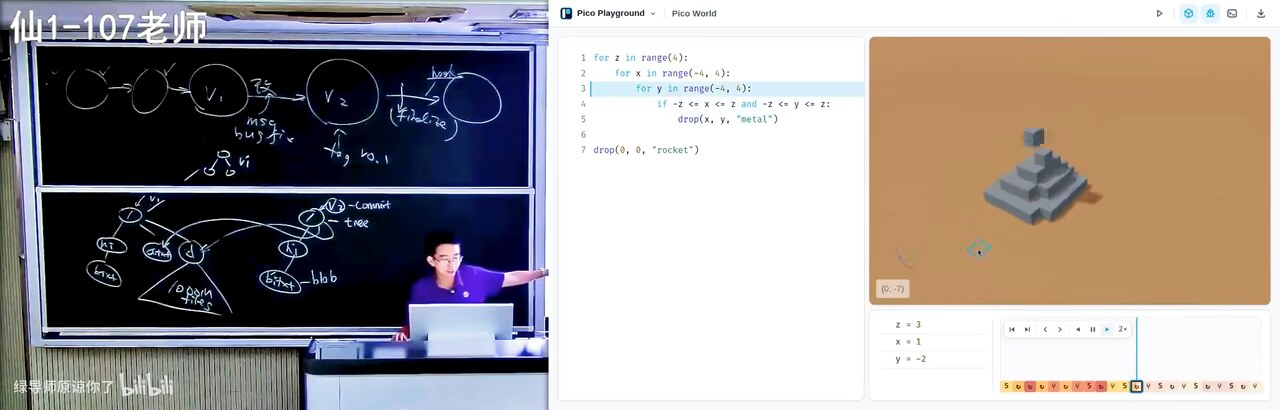
\includegraphics[width=\textwidth]{figures/fig_31_pico_world_3d.jpg}
\caption{Pico World：三重 for 循环调用 drop(x,y) 搭建体素世界，可调试可回放\vtag}
\end{figure}
\srcnote{01:23:00--01:23:14}

\subsection{“愿意学懂”成了有价钱的品质}

工具成本归零后，剩下的稀缺品质是什么？讲者给出求职市场的观察：一旦有人学会把细节做好，招人单位就用这个标准衡量所有人；“大学里没训练过，真上了战场就都得死”；很多老师对着课本讲一遍，而真正好的项目“打开都没打开过”——“上课耽误学习是真实存在的”，他的版本是：不打开好项目、不消化细节才耽误学习。好消息（在他的价值判断里）是真正学懂与成绩正相关。他自估那套完整可视化教学框架只花了两天碎片时间——包括视觉调整，“做这些事情已经没有任何成本了”，并自嘲“所以我马上就淘汰了”。

\begin{figure}[H]
\centering

\includegraphics[width=\textwidth]{figures/fig_32_learn_to_understand.jpg}
\caption{求职判断：把细节做好的 bar 不断抬升；愿意学懂成为真正有价值的品质（讲者观点）\vtag}
\end{figure}
\srcnote{01:26:15--01:26:29}

\subsection{本章小结}
教学工具人人可造之后，区分度回到学习者本身：注意力、品位、愿意学懂。讲者把这些判断都标注为自己的观察而非测量结论；接下来收束全课——所有内容其实都从一句话推出。

\section{总结与延伸：项目是由 Atomic Change 推进的快照}

\subsection{讲者的收束}

“虽然我好像在讲 Git，其实我讲的是 best practice。”而所有 best practice 背后还有一句更小的话：

\begin{equation}
V_n \;=\; V_0 \circ \Delta_1 \circ \Delta_2 \circ \cdots \circ \Delta_n,\qquad
\text{每个 }\Delta_i\text{ 只承载一个意图}
\end{equation}
式中 \(V_0\) 为初始状态，\(\Delta_i\) 为第 \(i\) 个 atomic change，\(\circ\) 表示状态依次推进。项目 = 由 atomic change 推进的快照，可分支、可合并——分支上失败的尝试可以安全扔掉，成功就合并进来，多条主线可以并行推进而互不干扰。

\begin{importantbox}{项目管理的本质}
人类没有办法处理一团混沌：很多需求、很多代码、一次做一大波，改着改着就与这处冲突、与那处冲突。自然的做法是把需求分解成可以理解、可以审计的小任务——一个 change 对应一个意图，出了问题才能单独解释、验证、撤销；这也正是 atomic change 一词的全部含义。
\end{importantbox}

推论链环环相扣：人类无法处理一团混沌（同时改好几个地方，改着改着就乱了），所以必须把需求分解成可以理解、可以审计的小任务；小步提交让 bisect 可行、冲突范围小、合并容易；linear history 之所以流行，是因为它让历史易追溯、对 cherry-pick/blame 友好，AI 维护项目也省 token。在“无限大能力的模型到来之前”，这条法则对人与 AI-native 团队同样成立。

\begin{figure}[H]
\centering
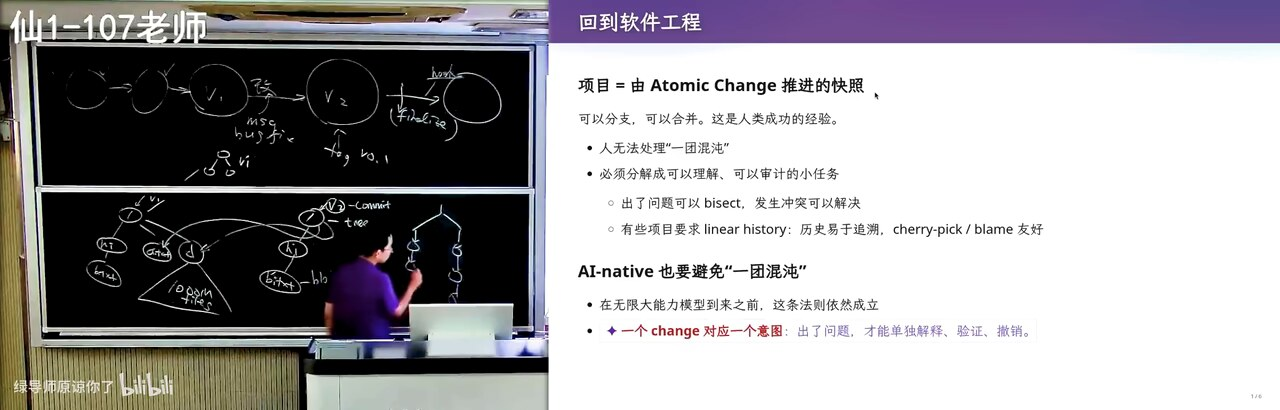
\includegraphics[width=\textwidth]{figures/fig_38_atomic_change.jpg}
\caption{回到软件工程：项目 = 由 atomic change 推进的快照；AI-native 也要避免一团混沌\vtag}
\end{figure}
\srcnote{01:35:00--01:35:14}

\subsection{讲者的工程工作流（口述复盘）}

架构设计阶段单线程：用一个高智力模型反复讨论、直到收敛，把设计落到文档、规则与示例（比如测试要做到什么程度）；仍要学操作系统、编译原理、数据库，“这里有人类积累的好设计”。组件接口尽量定为 pure function——可视化状态是程序状态的纯函数，全局互相影响的状态注册到一个全局处，核心共享状态只有十几行、组装十几行，其余全是黑盒；并要求 agent 设计新组件时“禁止看任何函数的实现，只看接口”，一个 playground 几万个 token 就能做完。架构定型后再开并行实现，终端数量他刻意控制在 n$\le$ 3 个；\texttt{AGENTS.md} 写明协作规则：不调用视觉模型自查（费 token）、不自己开浏览器——他在旁边放一块屏跑实时刷新，人肉验收，“哪里不满意就骂它”。讲者判断这类是“agent 能力之内的项目”，并且 agent 能力会不断增长，越来越多项目能以“轻量讨论 + 放手完成”的方式交付。

\begin{figure}[H]
\centering
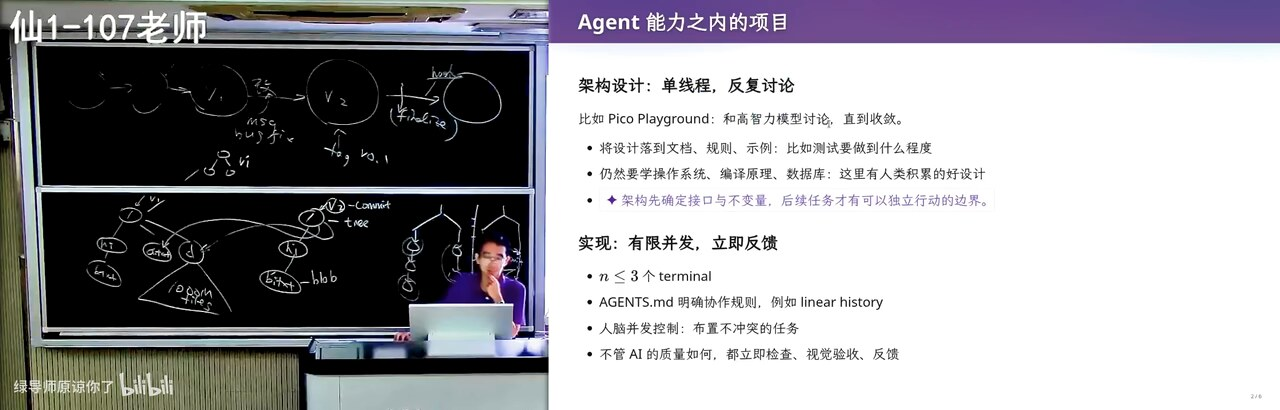
\includegraphics[width=\textwidth]{figures/fig_39_agent_project.jpg}
\caption{Agent 能力之内的项目：架构单线程讨论、实现有限并发（n$\le$ 3 终端）、AGENTS.md 定规则\vtag}
\end{figure}
\srcnote{01:36:45--01:36:59}

\subsection{整理者的综合}

把本课压成三句话：\textbf{（1）版本管理的问题只有一个}——目录在任意过去的样子能否保留、比较、恢复；快照 + 共享节点 + 记录来路是它当前最好的解。\textbf{（2）best practice 不是规矩而是定理}：小步原子提交、可构建的快照、描述动机的消息、忽略不该入库之物、不重写他人依赖的历史——每一条都能从“历史是审计对象”推出，也能从一次事故反推。\textbf{（3）AI 改变了分工没改变目标}：agent 生成、检查、重写历史都可以做，但“什么该发生”的判断（冲突怎么解、规则名大小写、要不要空提交）仍要求人保留注意力；路牌原则同时是好的工具设计与好的学习方法。

讲者留下的开放问题：如果 agent 快了一千倍（幻灯片：Agent 可以 1000X 更快地生产代码），仓库流程、review 粒度与协作约定该长成什么样？——“我们可以下一节课再来讨论。”

\subsection{拓展阅读}
\begin{itemize}
\item ProGit（讲者点名；视频 33:40）——Git 官方风格的入门书。
\item Conventional Commits 规范页（视频 87:30）——type 前缀约定的原始文本。
\item learn git branching（视频 68:45）——交互式分支演练。
\item Herbert Simon, \emph{The Structure of Ill Structured Problems}（1973）；\emph{How People Learn}（2000）——课首两处的引用来源。
\end{itemize}

%% --- 正文内容结束 --- %%

\end{document}
